\pdfoutput=1

\documentclass{article}

\usepackage[preprint]{tmlr}

\usepackage{amsmath,amssymb,amsfonts}
\usepackage{booktabs}
\usepackage{graphicx}
\usepackage{hyperref}
\usepackage{xcolor}
\usepackage{multirow}
\usepackage{microtype}

\renewcommand{\arraystretch}{1.3}
\emergencystretch=1.5em

\title{Mechanistic Validity Audit: Lookback Mechanism for Belief Tracking}

\author{\name Elliot Tower \\
      \email elliot@elliottower.ai}

\begin{document}
\maketitle

\begin{abstract}
Causal findings in mechanistic interpretability carry specific labels---belief tracking, planning, deception---whose specificity is rarely tested. \citet{prakash2025lookback} report a ``lookback mechanism'' in Llama-3-70B-Instruct that tracks characters' beliefs through pointer dereference via attention, identifying low-rank subspaces at three layer ranges that carry belief content when swapped between stories. We apply the 36 criteria of the Mechanistic Validity framework and identify six untested assumptions, most critically that the CausalToM generator drops the \texttt{causal\_event} field its own templates define, so every story on which the subspaces were identified has belief equal to reality. The paper reports true- and false-belief experiments on BigToM, and also reports that the subspaces are not shared between the two datasets, so the localized subspaces themselves were never tested against a false belief. Fifteen experiments were pre-registered in timestamped amendments; twelve completed, three of them overturning our own predictions. (1)~The answer subspaces at L38 and L52 transfer to stories where belief diverges from reality (IIA $= 0.975$ each) and to observability-mediated knowledge ($0.988$ and $0.975$), overturning our pre-registered prediction that they would not; L53 does not follow them ($0.388$ and $0.213$). Question framing modulates transfer: belief questions give IIA $= 1.0$ while reality-state questions give $0.82$--$0.92$ over the same story pairs, a reliable reduction that does not abolish transfer. (2)~A cross-model mismatch test on Qwen2.5-14B-Instruct confirms the answer lookback's dependency structure transfers (singles near zero, pair at $1.0$) while the binding mechanism shows a structurally different pattern---partial transport that full-residual patching cannot detect. (3)~That test is a complete two-player coalition function, so the interaction between its token groups is exact: the binding protocol yields a parity function at layers 24--34, with both order-1 coefficients exactly zero and all non-constant energy at order~2, while the answer protocol yields a conjunction at layers 32--38 ($w_2 = +0.249$ against a ceiling of $+0.25$). A summary reporting marginal contributions assigns the binding run two zeros. The two protocols differ in generator, layer range and the size of the patched span, so the sign difference is a difference between protocols as run and is not yet attributable among those three. (4)~The matched-rank random-subspace comparison the audited work omits is supplied here: across the six identified subspaces, none of 350 random draws of the same rank from the same basis reaches the identified interchange accuracy, so baseline separation (M2) is met and the causal rungs are open. All readings nonetheless stay at ``Causally Suggestive'', held there by cross-distribution generalization (E1), since every story follows one template, and by specificity (I4), where cross-task transfer and distractor fragility point in opposite directions. We propose the term \emph{perspective-indexed entity binding}.
\end{abstract}

\noindent\textbf{Keywords:} mechanistic interpretability, validity, belief tracking, interchange interventions, replication


\section{Introduction}
\label{sec:intro}

Mechanistic interpretability assigns causal roles to model components via interchange interventions---swapping internal representations between paired inputs \citep{geiger2021causal, vig2020investigating}. Successful experiments are labeled as ``the mechanism'' for a capability: induction heads for in-context learning \citep{olsson2022context}, the IOI circuit \citep{wang2023interpretability}, the ``lookback mechanism'' for belief tracking \citep{prakash2025lookback}. These labels carry validity assumptions---construct, measurement, internal, external, interpretive---that are rarely tested.

We audit \citet{prakash2025lookback}, who claim that large language models implement belief tracking via three ``lookback'' sub-mechanisms---binding (layers 33--38), answer (layers 52--56), and visibility (layers 10--31)---collectively described as ``pointer dereference via attention.'' We apply the 36 validity criteria and identify six untested assumptions.\footnote{We draw on three deposited frameworks: Mechanistic Validity \citep{tower2026mechval}, which provides the 36 criteria; Mechanistic Views \citep{tower2026mechviews}, which asks what \emph{kind} of claim a given method can support; and Mechanistic Reference \citep{tower2026mechref}, which asks whether a mechanism's name refers to anything the method can actually detect. Each is independently deposited; the audit's findings stand without them.} The claim rests on interchange interventions on 80 synthetic stories in Llama-3-70B-Instruct, pre-filtered to cases the model answers correctly, with qualitative replication in two other models. The three sub-mechanisms operate on different token types at different layer ranges, with per-layer subspace ranks from 3 to 19 singular vectors for the pointer concept and up to 320 for visibility (selected from a truncated SVD of the 8192-dimensional residual stream).\footnote{Ranks extracted from released results at \url{https://github.com/Nix07/belief_tracking} (commit \texttt{0579347e}); the SVD uses 500 components. See \texttt{reference/extracted\_results\_llama70b.json} in our repository.}

We produce a verdict on the five-tier scale (Proposed, Causally Suggestive, Mechanistically Supported, Triangulated, Validated) and pre-register fifteen experiments to test the gaps; three of four dissociation experiments overturn their predictions, each time strengthening the audited claim.

\paragraph{Contributions.}
(1)~A validity assessment against the 36 criteria, most critically showing that the CausalToM generator never instantiates the false belief its own templates encode, so the identified subspaces were localized without one, and fifteen pre-registered experiments testing the gaps.
(2)~A framing dissociation confirming belief-specific subspaces: belief questions give IIA $= 1.0$ while reality-state questions give $0.82$--$0.92$ over the same story pairs, and the subspaces generalize to genuine false beliefs (IIA $= 0.975$) and observability-mediated knowledge (IIA $= 0.988$).
(3)~An exact interaction decomposition of the cross-model test, which finds the two protocols carrying pairwise interactions of opposite sign, each saturated at the bound the design admits, and identifies the crossed design that would attribute the difference.
(4)~A verdict per reading rather than one for the claim, with cross-distribution generalization (E1) and specificity (I4) identified as the gates holding every reading at ``Causally Suggestive'', and a revised term: \emph{perspective-indexed entity binding}.


\section{Validity Assessment}
\label{sec:validity}

Table~\ref{tab:validity} and Figure~\ref{fig:validity_grid} summarize the assessment.

\subsection{Construct validity}

\paragraph{No discriminant validity (C4).}
No task where the lookback pattern should be absent is tested. Candidate negative controls: factual recall without belief tracking, simple copying, single-character stories, non-ToM multi-step retrieval. If the pattern appears on all of these, it is attention-mediated retrieval, not belief tracking.

\paragraph{No complementation test (C6).}
The mechanism is carved into three named sub-mechanisms---binding, answer and
visibility---and each is tested alone. Single-stage interventions cannot separate three
distinct complementation groups from one group whose members share a role: that comparison
requires ablating two stages and reading their joint effect against a composition rule. We
pre-registered the test as Experiment~5 (cross-stage mediation); the run did not return
usable estimates, so the question stands open on our evidence as well as on the audited
paper's.

\paragraph{No convergent evidence (C3).}
Interchange interventions on residual stream vectors carry the argument, and subspace identification uses the same framework (SVD of intervention-site activations, then a binary mask over singular vectors trained to maximize the counterfactual logit). Appendix~L adds one weight-space measurement: the column-normalized query projection is projected onto the identified subspace basis, reshaped per head, and reported as a per-head Frobenius norm, with the same computation repeated for value projections (Figures~19 and~20). It does not converge on the subspace result independently, because the basis it projects onto is the mask's output, so a subspace selected for the wrong reason yields head norms selected for the wrong reason. No baseline accompanies it---no matched-rank random subspace, no null distribution over heads---and no test accompanies the figures, which are read as agreeing with the intervention result. No attention pattern analysis is reported. The qualification on independent
probing is that the ordering-ID construct the mechanism is built on comes from
\citet{dai2024representational}, who identify a low-rank subspace encoding ordering by PCA
and confirm it by causal editing, and whom the audited paper cites. That is a second method
family bearing on the construct, though not on the lookback subspaces themselves, which rest
on interchange alone.

The paper's evidence occupies a single level \citep{tower2026mechviews}: the role level, where mechanisms are functional roles validated by intervention success. The subspace identification (DCM) parameterizes the search at a finer grain---selecting directions on the Grassmannian $\text{Gr}(k, d)$---but validates only by IIA, which is a role-level criterion (does the interchange produce the predicted output?). Confirming a genuine subspace claim requires convergent evidence from weight-space analysis: which attention heads implement the retrieval, whether the identified subspace is stable across random seeds, and whether it occupies a consistent location on the Grassmannian across models. The paper provides none of these.

Eleven experiments across three models and dozens of layer-concept combinations look like massive convergent evidence. They are one measurement family applied repeatedly. Quantity of replications within one method does not substitute for an independent method.

\paragraph{Construct import.}
``Belief tracking'' imports cognitive-science vocabulary---Theory of Mind \citep{premack1978chimpanzee}, false-belief attribution \citep{wimmer1983beliefs}---without validating the transfer. The model passes a behavioral ToM test; the internal mechanism gets cognitive-science labels. Behavioral equivalence does not entail mechanistic equivalence \citep{ruis2025reevaluating}.

\subsection{Measurement validity}

\paragraph{No random subspace baseline in the audited work (M2, supplied here).}
SVD followed by L1-regularized binary mask selection produces per-layer subspaces of varying rank---typically 3 to 19 singular vectors for the pointer concept, from a truncated SVD of the 8192-dimensional residual stream. No random subspace of matched rank is tested for comparable IIA. In several experiments, subspace IIA approaches full residual stream IIA (e.g., 0.925 vs.\ 1.0 at layer 38 for the pointer concept), suggesting the subspace captures most task-relevant signal. The visibility lookback is particularly striking: the selected ``subspace'' uses 160--320 of 500 SVD components (32--64\% of the truncated basis, 2--4\% of the full residual stream), where a weaker L1 penalty ($\lambda = 0.03$ vs.\ $0.1$) lets the optimizer retain most candidate dimensions. At early layers, the selected subspace achieves higher IIA than the full 500-component basis (e.g., 0.90 vs.\ 0.175 at layer 7), suggesting remaining SVD components destroy counterfactual behavior---consistent with meaningful directional selectivity or optimization artifacts.

\paragraph{Method vacuousness (M2, continued).}
\citet{sutter2025vacuous} demonstrated that unconstrained DAS achieves 100\% IIA on randomly initialized models: a method that succeeds on every system, including random ones, has zero discriminative power. DCM constrains the search to binary masks over a fixed SVD basis rather than arbitrary rotations, so it is more constrained than unconstrained DAS. Whether these constraints are sufficient to avoid vacuousness is an empirical question: if DCM finds low-rank subspaces with high IIA on a randomly initialized model, the method inherits the Sutter problem despite its constraints. We include this as a control in Experiment~2.

\paragraph{No effect size calibration (M1).}
IIA is the sole metric, reported without confidence intervals or statistical tests. For $n = 80$, the standard error on IIA is at most ${\sim}5.6$ percentage points ($\sqrt{0.5 \cdot 0.5 / 80}$, the maximum at $p = 0.5$), placing values below ${\sim}0.60$ within noise of chance for a binary outcome.

\paragraph{Selection on the dependent variable (M7).}
All CausalToM examples were pre-filtered to cases the model answers correctly on both clean and counterfactual prompts. The analysis conditions on the output, then attributes a mechanism to the internal process. Failure cases are excluded. The codebase does generate a train/eval split (80 stories each; \texttt{scripts/patching\_scripts/run\_patching\_exp\_utils.py:465}): the binary mask is optimized on training stories and IIA is reported on held-out validation stories. However, the SVD basis---which defines the candidate directions the mask selects from---is pre-computed offline (\texttt{svd/} directory, not committed to the repository), with no documentation of a held-out procedure. The evaluation is therefore out-of-sample relative to the mask but likely in-sample relative to the feature space.

\subsection{Internal validity}

\paragraph{Full-vector confound (I7).}
Interchange interventions swap the entire residual stream vector (or a large subspace), transferring all information at that position, including the hypothesized ``pointer'' along with everything else. Two interpretations are consistent: (a) the model uses a specific pointer structure and the swap transfers it, or (b) the model uses any information in the residual stream and the swap includes it. Interpretation (b) makes no mechanistic claim beyond ``information flows through the residual stream.''

\paragraph{No epistatic interaction test (I9).}
The three sub-mechanisms are tested independently. Whether disrupting binding changes the answer lookback's behavior beyond the additive prediction is untested. Non-additive interaction would support a single staged mechanism; additive independence would support three separate processes sharing a label.

\paragraph{No offset coupling test (I12).}
The audited results come from one checkpoint. Whether the components carrying the role at
this offset carry it earlier or later in training is not observable in the design, so a
component that holds the role transiently and one that holds it throughout are
indistinguishable here.

\paragraph{No rescue reversibility (I10).}
The paper ablates the mechanism (showing necessity) but does not restore a corrupted component to test whether behavior recovers. Rescue experiments distinguish a causal bottleneck from a correlated side-effect.

\subsection{External validity}

\paragraph{Single template (cross-distribution generalization).}
All 80 stories follow the CausalToM template with fixed token positions, exactly two characters, and exactly two objects. No structural variation is tested.

\paragraph{No cross-task transfer.}
The paper tests model generality (Gemma-3-27B, Qwen-2.5-14B) without task generality: different story formats, naturalistic text, multi-step reasoning with belief tracking as one component.

\paragraph{No graded response.}
No partial ablation of the subspace is tested for proportional degradation. A dose-response curve would distinguish a sharply localized mechanism from diffuse information storage.

\paragraph{No novel prediction.}
The mechanism is characterized post hoc, with no new behavioral prediction derived from the mechanistic account and tested on held-out data.

\subsection{Interpretive validity}

\paragraph{Referential inflation (V1, V4).}
The rating here rests on the paper's scope language rather than on its central analogy. Calling the operation a ``pointer dereference'' is a metaphor, and a defensible one: it names a real pattern of attention-mediated retrieval, and a reader is not misled by it. What the evidence does not license is the surrounding quantification---``pervasive,'' ``a fundamental role in in-context reasoning,'' and the conclusion that the work has ``mapped the end-to-end underlying mechanism.'' Those are claims about scope, made from 80 templated stories in one model family, and they are what V1 and V4 record. For completeness the analogy's content: allocate a reference, store an address, follow the reference, retrieve a value. The evidence shows attention-mediated information flow between token positions. Consider three statements of the same result:

\begin{quote}
\emph{What the experiment shows.} Replacing the residual stream vector at the final token position with the vector from a counterfactual story changes the model's answer to match the counterfactual, for a 19-dimensional subspace of a 500-component SVD basis, at layers 52--56, on 80 template-matched stories.

\emph{What this licenses.} Information at this position and layer range is causally necessary for producing the belief-consistent answer.

\emph{What the paper claims.} The model implements pointer dereference: it stores an address, follows the reference, and retrieves the payload.
\end{quote}

The gap between the second and third statement is not supplied by any experiment---it is supplied by the vocabulary. Substituting ``pointer'' $\rightarrow$ query vector, ``address'' $\rightarrow$ key vector, ``payload'' $\rightarrow$ value content, ``dereference'' $\rightarrow$ attention, the finding reduces to: the model uses attention to retrieve information from earlier tokens. This is what attention does by construction. \citet{tower2026mechref} calls this pattern \emph{referential inflation}: the labels carry referential content---computational specificity---that the method cannot detect. Strip the metaphor and the level jump becomes visible.

\paragraph{No falsification target.}
No result would have falsified the lookback hypothesis as stated. High IIA supports it, low IIA means ``the mechanism does not operate here,'' and matched full-vector and subspace IIA means ``the subspace captures the information.'' Every outcome confirms.

\paragraph{The third-answer result.}
The paper's strongest evidence is the answer pointer experiment (Figure 4b): swapping the ``pointer'' while preserving the ``payload'' produces a third answer~$C$ distinct from both the original answer~$A$ and the counterfactual answer~$B$. This demonstrates decomposable internal structure---a random-noise perturbation would degrade $A$, not produce a coherent alternative.

The structure, however, is predicted by the attention mechanism itself. QK circuits determine \emph{where} to attend (the pointer); OV circuits determine \emph{what} to retrieve (the payload). Swapping directions that alter QK routing makes the model attend to a different earlier position and retrieve whatever content is stored there via OV---producing a coherent third answer corresponding to the content at the redirected position. Every transformer attention head exhibits this pointer-payload decomposition by construction; the question is whether the specific subspace identified by DCM captures belief-specific routing or generic QK structure.

We confirm the decomposable structure as genuine and test the belief-specificity question in Experiments~2 and~3 (Section~\ref{sec:experiments}). Experiment~2 includes a specific test: if random subspaces of matched rank also produce coherent third answers at above-chance rates, the decomposition is a property of the SVD basis geometry, not of the identified directions. We define ``coherent'' quantitatively before seeing the data: a third answer counts as coherent if it is a token from the story's entity vocabulary (character names, objects, locations) distinct from both $A$ and $B$. The coherent-third-answer rate on the identified subspace must exceed the rate on random subspaces ($p < 0.01$, rank test) to support directional specificity.

\subsection{Summary}

\begin{table}[t]
\centering
\caption{Validity assessment against the 36 criteria of \citet{tower2026mechval}. Two criteria fail outright (V1: level declaration, V4: unlicensed labeling). Criteria not discussed individually are rated in the supplementary audit document. C6 (complementation validity) and I12 (offset coupling) entered the framework after the audit was pre-registered and are scored here against the same record; see Amendment~11.}
\label{tab:validity}
\begin{tabular}{lcccc}
\toprule
Category & Confirmed & Partial & Not met & Fails \\
\midrule
Construct (C1--C6) & 1 & 2 & 3 & 0 \\
Measurement (M1--M7) & 0 & 2 & 5 & 0 \\
Internal (I1--I12) & 1 & 2 & 9 & 0 \\
External (E1--E6) & 0 & 2 & 4 & 0 \\
Interpretive (V1--V5) & 0 & 2 & 1 & 2 \\
\midrule
\textbf{Total (36)} & \textbf{2} & \textbf{10} & \textbf{22} & \textbf{2} \\
\bottomrule
\end{tabular}
\end{table}

\begin{figure}[t]
\centering
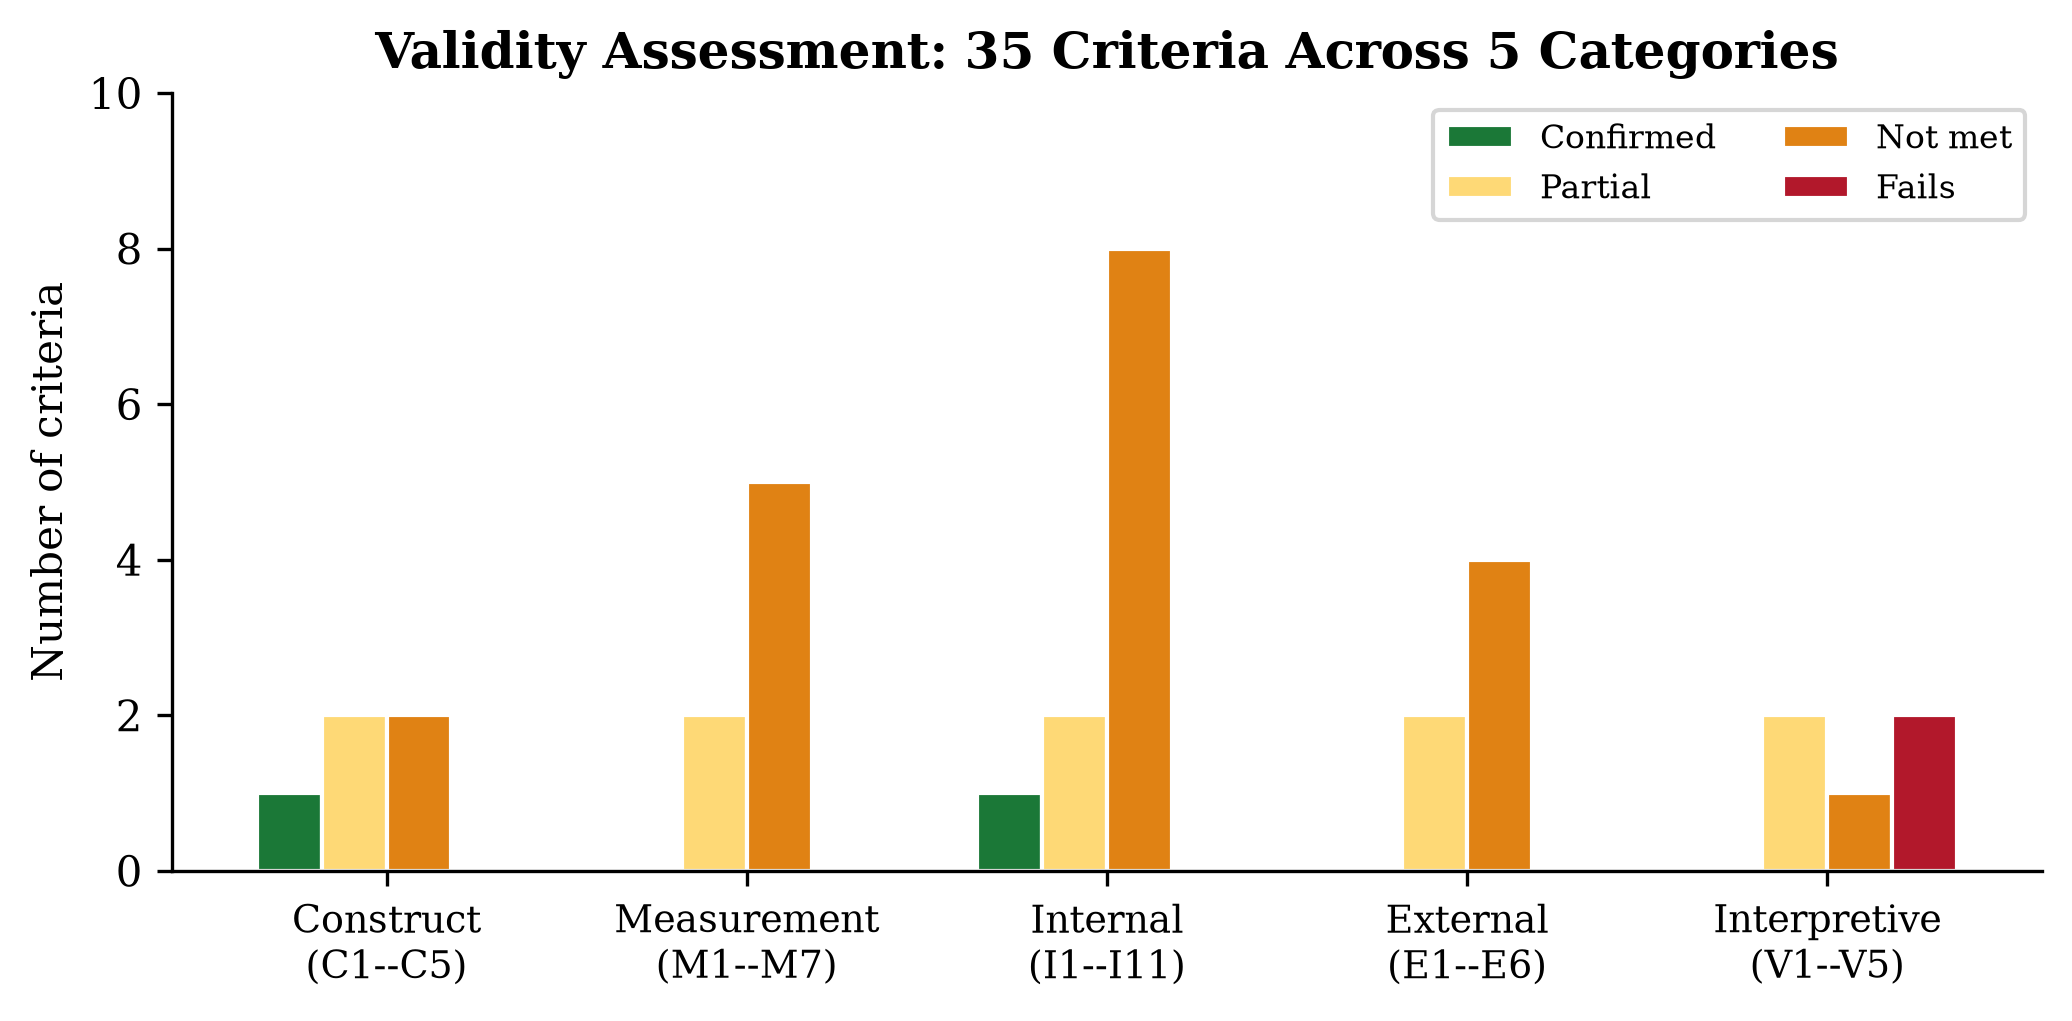
\includegraphics[width=0.85\textwidth]{figures/fig6_validity_grid.pdf}
\caption{Validity assessment across 36 criteria grouped into five categories. Most criteria are ``not met'' (22/36), reflecting the paper's minimal reporting of measurement and internal validity evidence. Two criteria fail outright (V1: level declaration, V4: unlicensed labeling). The ten partial ratings correspond to criteria where the paper provides some relevant evidence without meeting the full standard.}
\label{fig:validity_grid}
\end{figure}

The ladder gates are conjunctive. Causally Suggestive requires necessity (I1) together with baseline separation (M2); Mechanistically Supported adds sufficiency (I2), cross-distribution generalization (E1) and alternative-mechanism exclusion (I4). The paper establishes necessity through ablation and reports no comparison against a matched random subspace, so on its own evidence M2 is unmet and every causal rung is unreachable. We supply that comparison in EXP2 (Section~\ref{sec:results}) and M2 is met on the measurement. The gates that then bind are E1, since every story follows one template, and I4, since no rival account of the same transfer has been excluded.


\section{The Unity Problem}
\label{sec:unity}

The paper treats three ``lookback mechanisms'' as instances of a single computation. They operate at non-overlapping layer ranges, on different token types, with per-layer subspace ranks that differ by an order of magnitude (3--10 for binding vs.\ 160--320 for visibility; Table~\ref{tab:unity}).

\begin{table}[t]
\centering
\caption{The three ``lookback mechanisms'' differ in every measurable property. Subspace ranks are per-layer (selected via L1-regularized binary mask over SVD components) and vary across layers within each mechanism. Ranks extracted from released results at commit \texttt{0579347e}; exact values depend on layer and L1 weight ($\lambda = 0.1$ for binding/answer, $\lambda = 0.03$ for visibility).}
\label{tab:unity}
\begin{tabular}{lccc}
\toprule
Lookback & Layers & Tokens & Per-layer rank \\
\midrule
Binding & 33--38 & State tokens & 3--10 \\
Answer & 52--56 & Final token (``:'') & 18--19 \\
Visibility & 10--31 & Visibility sentence & 160--320 \\
\bottomrule
\end{tabular}
\end{table}

The unity claim rests on shared vocabulary: all three involve ``lookback'' (attention to an earlier token) and ``dereference'' (retrieval at the attended position). This describes the attention mechanism itself---every QK circuit attending to a previous position and retrieving content through OV fits the definition. The assumption is also unresolved in the source discipline: \citet{apperly2009humans} proposed that human belief tracking involves two distinct systems, and the strongest evidence for a single automatic system \citep{kovacs2010social} did not replicate \citep{phillips2015second}.

The critical test is coupling: if binding (layers 33--38) is disrupted, does the answer lookback (layers 52--56) degrade? Sequential dependence would indicate one staged mechanism. Independent disruptability would indicate separate processes sharing a naming convention. The paper does not perform this test.


\section{Pre-Registered Experiments}
\label{sec:experiments}

An audit of another group's work can easily become a post-hoc narrative: run many experiments, report the ones that tell a story. We pre-register six experiments and commit predictions before seeing data so the reader can verify which outcomes we expected and which surprised us. Three experiments are primary (run first), three secondary (run if primary experiments succeed). All use Llama-3-70B-Instruct via NNsight, reproducing the original setup. All $p$-values are Benjamini-Hochberg corrected across the six experiments. The pre-registration was committed at tag \texttt{prereg-amendment-5} before results were computed; subsequent amendments (7--9) are SHA-tagged in \texttt{AMENDMENTS.md}.

\subsection{Held-out basis validation (M2, M7)}

The original codebase validates the binary mask out-of-sample (mask trained on 80 stories, IIA evaluated on a separate 80). The SVD basis itself, however, is pre-computed offline with no documented held-out procedure. This experiment tests whether the reported subspaces generalize when the SVD basis is also computed on disjoint data. Protocol: partition a larger pool of CausalToM stories (320+, generated from the same templates) into three non-overlapping sets---SVD estimation, mask training, and IIA evaluation. Recompute the SVD on the estimation set, fit the binary mask on the training set using the original hyperparameters, and evaluate IIA on the held-out evaluation set. Repeat for each layer $\times$ concept combination.

\paragraph{Pre-committed interpretations.} If IIA on held-out data matches the released values within $\pm 0.05$ (4 examples on an 80-story evaluation set), the SVD-basis-leakage concern is closed and we report M7 as satisfied for the feature space. If IIA drops substantially (below 0.5 or below the 95th percentile of the random subspace distribution from Experiment~2), the reported subspaces are artifacts of basis overfitting and the claim requires recomputed SVD with proper held-out evaluation.

\subsection{Matched-capacity controls (M2)}

Two controls with matched optimization budget, evaluated on the same held-out set from Experiment~1:

\paragraph{Random subspace baseline.} For each layer's identified subspace of rank $r$, sample 200 random $r$-of-500 index sets from the same SVD basis (uniformly without replacement, matching the paper's binary-mask method). Compute IIA for each on the held-out evaluation set. The identified subspace should rank in the top 1\% ($p < 0.01$, one-sided rank test with corrected $p = (k + 1)/(n + 1)$). This is a floor control: the identified subspaces are optimized to maximize IIA while random selections are not, so the identified subspace beating random draws is expected. Additionally, we record the coherent-third-answer rate (see Section~\ref{sec:validity}) for each random subspace to test whether the decomposable structure is direction-specific.

\paragraph{Shuffled-label control.} For two primary layer-concept combinations (one binding: \texttt{binding\_lookback/address\_and\_payload} at layer 34; one answer: \texttt{answer\_lookback/pointer} at layer 52), re-run the SVD + mask selection procedure with identical hyperparameters (Adam, $\text{lr} = 0.1$, L1 weight matching the original) on 100 permutations of the belief labels---shuffling which story's belief state serves as source for interchange intervention. Crucially, shuffled masks are \emph{trained} on shuffled assignments but \emph{evaluated} on real counterfactual targets (held-out set). The real-label subspace should beat the shuffled-label distribution ($p < 0.01$, rank test). The remaining four layer-concept combinations are tested as exploratory with 20 permutations each ($p$-floor $= 0.048$).

\paragraph{Vacuousness control.} Apply the DCM procedure (SVD of activations, binary mask optimization with identical hyperparameters) to a randomly initialized Llama-3-70B. If DCM finds low-rank subspaces with IIA exceeding chance, the method inherits the \citet{sutter2025vacuous} vacuousness problem despite its constraints, and the subspace identification on the trained model is uninformative.

\paragraph{Pre-committed interpretations.} If real-label subspaces beat both random and shuffled-label baselines on held-out data, M2 is satisfied and the belief-specificity concern narrows to the task-generality question (C4, Experiment~3). If the vacuousness control produces high-IIA subspaces on the random model, DCM lacks referential content and the subspace results are methodologically void regardless of other outcomes. If shuffled-label subspaces achieve comparable IIA, the mask selection captures generic high-variance directions rather than belief structure, and the claim requires revision. If both shuffled and random subspaces approach the identified subspace's IIA, the subspace identification adds no information beyond dimensionality matching. Additionally, for the third-answer test: if random subspaces of matched rank produce coherent third answers (story-vocabulary tokens distinct from both original and counterfactual answers) at rates comparable to the identified subspace, the decomposable structure is a property of the basis geometry rather than of the identified directions.

\subsection{Task-specificity controls (C4)}

Run the interchange intervention protocol on programmatically generated stories (120 per condition) across four conditions that isolate binding and belief attribution:

\begin{enumerate}
\item Echo/copy (no binding, no belief): ``Alice said: `the X is in loc1.' What did Alice say?''---pure retrieval, the strong control.
\item Entity tracking (binding, no belief): ``Alice put X in loc1. Bob moved X to loc2. Where is X?''---a weak control, as the authors' own work predicts the pattern may appear here.
\item True-belief matched stories (binding, minimal belief): same CausalToM structure but the character's belief matches reality.
\item First-order false belief: standard CausalToM (the original task).
\end{enumerate}

Use the same layer ranges, subspace dimensions, and IIA metric across all conditions.

\paragraph{Pre-committed interpretations.} If the lookback pattern is absent on echo/copy and entity tracking but present on false belief, C4 is satisfied: the subspace captures belief-specific structure. If the pattern appears on entity tracking but not echo/copy, the mechanism is entity-state retrieval rather than belief tracking---a substantive correction of the interpretive claim, consistent with the authors' own entity-tracking prior work. If the pattern appears on all conditions including echo/copy, it is generic attention-mediated retrieval, not a belief-tracking mechanism.

\subsection{Compositional generalization (C3, C5)}
\label{sec:composition}

Correct outputs across story variations (behavioral systematicity) do not entail compositionally structured internal representations (representational systematicity). The Lookback paper shows the former and infers the latter. CausalToM uses exactly two characters, first-order beliefs, and a single story template. If the lookback mechanism is a genuine compositional representation of belief, it should extend to structurally novel cases. If it is a template-matched retrieval circuit, it will not.

That prediction has since been tested at a scale this audit cannot reach.
\citet{gurarieh2025mixing} evaluate the positional mechanism across nine models and ten
tasks and report that it does not generalize beyond settings with two or three entity
groups, offering lexical and reflexive retrieval as alternatives. Their result is behavioral
systematicity on the template without the representational systematicity that would carry
it off the template. We registered a compositional generalization test of our own, it was
superseded in print before we ran it, and we defer to the larger study. The paper is not silent
here either: Appendix~O reports behavioral evaluations on three character-object-state triples,
where all tested models succeed without visibility and none consistently succeeds with it, and
interchange interventions on the no-visibility condition in Qwen2.5-14B-Instruct.

The finding this audit reports is upstream of that one and does not depend on it. Whether
the mechanism generalizes is a question about a mechanism identified on a task; ours concerns
what the task contained. CausalToM's generator sets each character's belief equal to reality in
every pair, so the subspaces were localized without a false belief present. That holds whether
or not the positional account generalizes, and it would hold if \citet{gurarieh2025mixing} had
found the opposite.

The claim is about CausalToM and not about the paper as a whole. Appendix~M reports true- and
false-belief experiments on BigToM, described there as preliminary because BigToM ``lacks the
coherent structure necessary for causal analysis'' and not all CausalToM experiments could be
replicated on it. The same appendix reports that ``the subspaces encoding various types of
information are not shared between the two settings,'' and that the subspaces representing
pointer information at the final token ``differ significantly.'' By the paper's own account,
then, the false-belief evidence and the localized subspaces come from different settings, and
the subspaces this audit tests were identified where no false belief occurs. That is what
EXP14 supplies.

We test three axes of generalization (120 stories per condition):

\begin{enumerate}
\item \textbf{Character scaling.} CausalToM variants with 3, 4, and 5 characters. The binding lookback assigns ordinal indices (OI-1, OI-2) to two characters; a compositional scheme should extend to OI-3, OI-4, OI-5 with additional binding slots. A template-matched circuit will fail or degrade.
\item \textbf{Nested beliefs.} Second-order false belief: ``What does Alice think Bob believes Object2 contains?'' The binding lookback should extend to represent the nesting structure. If the same subspace handles first- and second-order beliefs at the same layers and ranks, the mechanism generalizes. If second-order requires different layers or substantially higher rank, the mechanism is first-order-specific.
\item \textbf{Content selectivity.} Human belief tracking is content-selective: people track false beliefs about presence differently than about absence \citep{schuwerk2015implicit}. We test beliefs about object location, object existence, character intentions, and character knowledge states. A unified mechanism should handle all content types with comparable IIA at comparable layers. Selective failure indicates a family of content-specific circuits rather than one mechanism.
\end{enumerate}

For each condition, we apply the full DCM procedure (SVD + binary mask optimization with the original hyperparameters) and compare: (a) whether the identified subspace overlaps with the original CausalToM subspace (cosine similarity between mask vectors), (b) whether IIA is comparable, and (c) whether the active layer ranges shift.

\paragraph{Pre-committed interpretations.} If the lookback pattern generalizes across all three axes with comparable IIA, layer ranges, and subspace dimensions, the representational systematicity claim is supported and ``belief tracking'' is a defensible label. If the pattern degrades on character scaling ($\text{IIA} < 0.5$ at 3+ characters), it is a two-character retrieval circuit. If it fails on nested beliefs, it is first-order-specific. If it shows content selectivity (different layers or subspaces for different belief types), ``lookback'' is a family name for multiple circuits rather than one mechanism---paralleling the dissociation observed in human belief attribution \citep{apperly2009humans}. Any of these outcomes is informative: degradation patterns reveal the mechanism's actual scope.

\subsection{Failure case analysis (I1)}
\label{sec:failure}

Run identical interventions on CausalToM stories where Llama-3-70B-Instruct answers incorrectly. The original paper excludes these by design. To ensure sufficient failures for a powered test ($n_{\text{fail}} \geq 20$), we generate a pool of 500+ CausalToM stories rather than using the original 80.

\paragraph{Pre-committed interpretations.} If lookback IIA is significantly lower on incorrect-answer cases ($p < 0.01$, permutation test), I1 is satisfied: the mechanism is absent when the model fails, supporting a causal role. If the lookback is present and intact on failure cases, it is a correlate of processing rather than a cause of correct answers. If the model's accuracy yields fewer than 20 failures even on 500 stories, we report the experiment as underpowered rather than drawing a conclusion.

\subsection{Cross-stage mediation (I9)}
\label{sec:mediation}

Test whether the binding and answer sub-mechanisms form a causal chain or operate independently, replacing the super-additivity test originally proposed.\footnote{Super-additive behavioral loss is ambiguous: independent stages in a serial pipeline can produce super-additive loss through off-distribution compounding, and components of one mechanism can appear additive.} Protocol: (a) intervene on the binding representation at layers 33--38; (b) measure the resulting change in the answer-pointer representation at layers 52--56; (c) intervene on the answer-pointer representation; (d) test whether the answer-pointer intervention mediates the binding intervention's effect on output. All interventions use mean-ablation (replacing the subspace component with its dataset mean) to keep activations on the data manifold.

\paragraph{Pre-committed interpretations.} If binding interventions propagate through the answer-pointer representation and the answer-pointer mediates binding's effect on output, the unity claim is supported: binding $\to$ pointer $\to$ answer forms a causal chain. If the stages independently affect output without mediating each other, they are separate processes sharing a label, and ``lookback mechanism'' as a unified construct is not warranted. If the mediation is partial, the truth is intermediate and we report the mediation proportion.


\section{Results}

\begin{table}[t]
\centering
\small
\caption{Experiment inventory. Identifiers, where each was registered, and status. Numbered
experiments belong to the pre-registered series; two further experiments were registered against
criteria rather than numbers and are named for what they test. Of the fifteen numbered experiments
registered before results, ten completed; with the two criterion-anchored experiments, twelve
completed in total. Six remain unrun and report no results here: EXP3, EXP16--EXP18 and
EXP21--EXP23.}
\label{tab:inventory}
\vspace{0.5\baselineskip}
\begin{tabular}{llll}
\toprule
Identifier & Registered in & Status & Reported \\
\midrule
EXP1 & Amendments 1--5 & complete & Section~\ref{sec:results} \\
EXP2 & Amendments 1--5 & complete & Section~\ref{sec:results} \\
EXP3 & Amendments 1--5 & not run & --- \\
EXP4--EXP9 & Amendments 1--8 & incomplete or withdrawn & Section~\ref{sec:partial} \\
EXP10--EXP11 & Amendment 8 & complete & Section~\ref{sec:results} \\
EXP12--EXP15 & Amendment 9 & complete & Section~\ref{sec:dissociation_results} \\
Cross-model & Amendment 10 (criterion E3) & complete & Section~\ref{sec:crossmodel} \\
Rescue & Amendment 10 (criterion I10) & complete & Section~\ref{sec:results} \\
EXP16--EXP18 & Amendment 12 & not run & --- \\
EXP19--EXP20 & Amendment 13 & complete & Section~\ref{sec:crossmodel} \\
EXP21--EXP23 & Amendment 13 & not run & --- \\
\bottomrule
\end{tabular}
\end{table}

The counts in the abstract refer to this table. ``Fifteen registered'' is the numbered series
EXP1--EXP15, frozen before any result it reports; ``twelve completed'' is the ten of those that
produced usable results together with the two criterion-anchored experiments. EXP19 and EXP20
were registered in Amendment 13, after the results of the numbered series, and are reported
here; the remaining experiments of Amendments 12 and 13 are listed for completeness and report
nothing.
\label{sec:results}

All experiments use Llama-3.1-70B-Instruct via NNsight/NDIF remote execution, applying the paper's released SVD bases and singular-vector masks to compute interchange intervention accuracy (IIA).

\subsection{Measurement validity: replication and baseline separation (EXP1--EXP2)}

\paragraph{EXP1: Positive control replication.}
We replicate the paper's interchange interventions on Llama-3.1-70B-Instruct (the paper uses Llama-3-70B-Instruct). L34 binding replicates within $\pm 0.05$ (IIA $= 0.988$ vs.\ paper's $0.963$). The answer subspaces show \emph{higher} IIA than reported: L38 $= 1.0$ (paper: $0.925$), L52 $= 1.0$ (paper: $0.775$), L53 $= 1.0$ (paper: $0.550$). L36 binding drops ($0.225$ vs.\ paper's $0.750$). L52 and L53's upward shifts suggest seed 10 underestimates typical IIA; multi-seed replication confirmed L53 variance spanning $0.55$--$0.99$ across seeds (Figure~\ref{fig:replication}).

\begin{figure}[t]
\centering
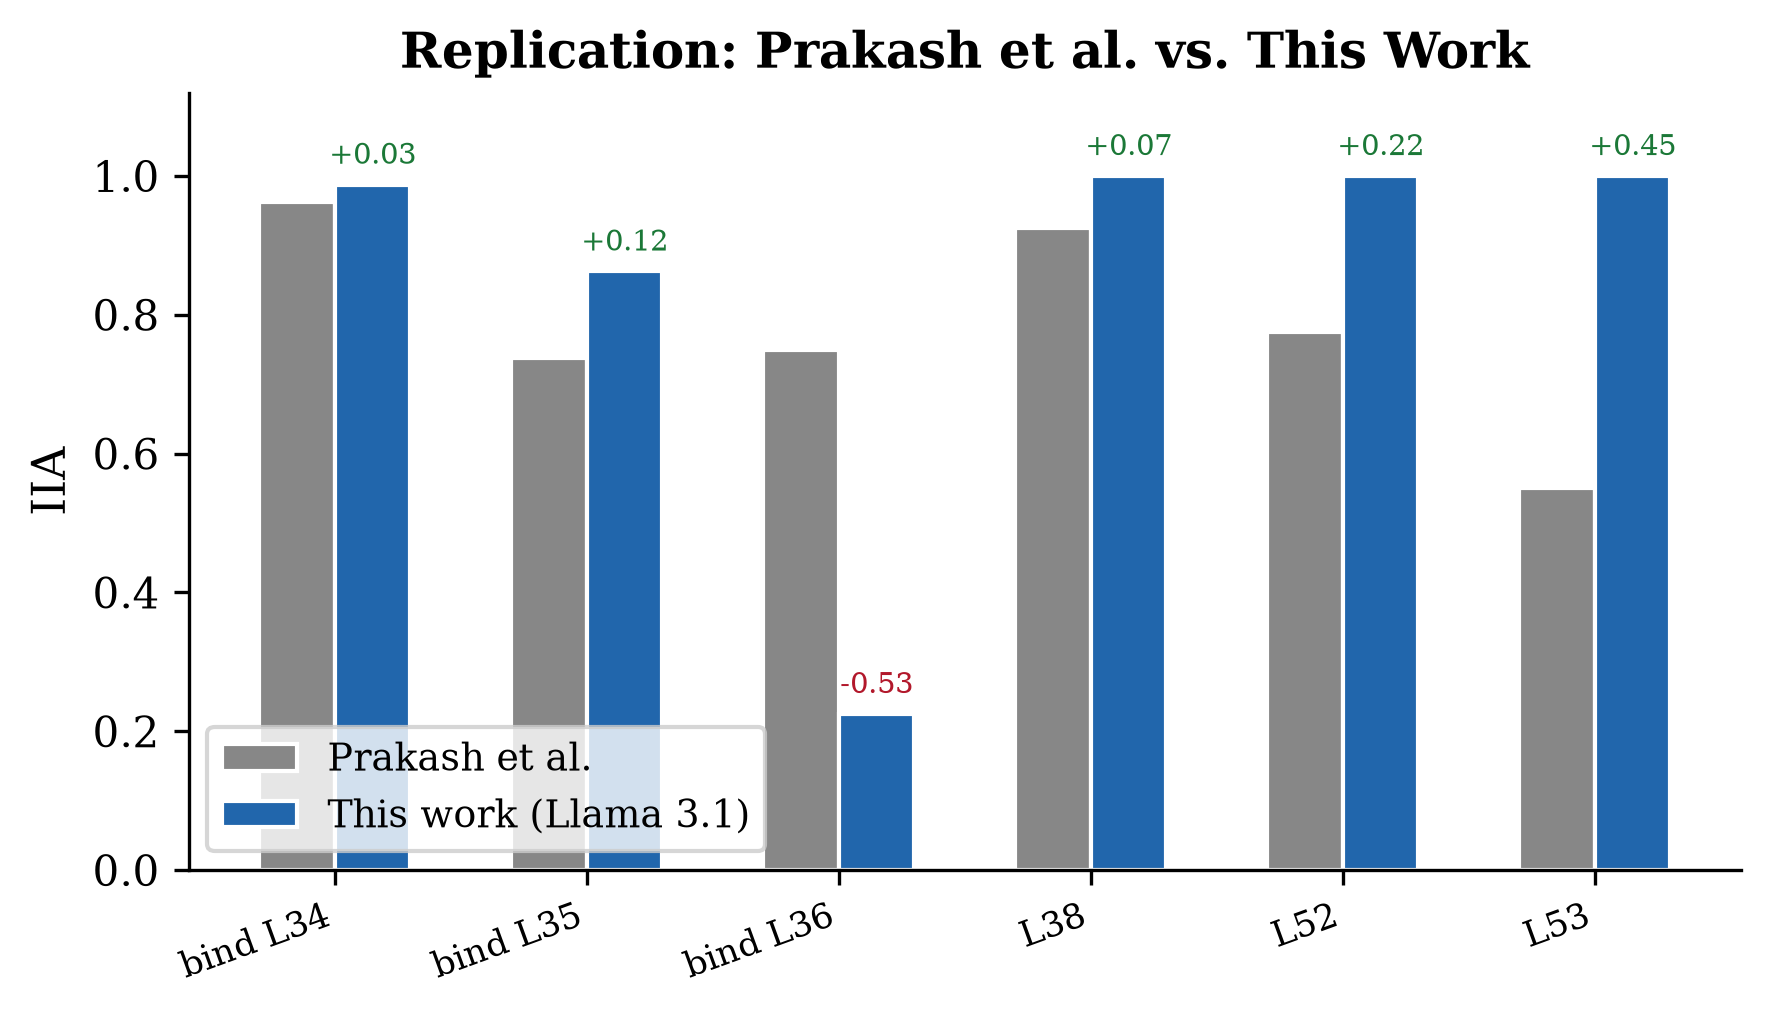
\includegraphics[width=0.85\textwidth]{figures/fig4_replication.pdf}
\caption{Positive control replication (EXP1). IIA for all six subspaces: Prakash et al.\ on Llama-3-70B-Instruct (grey) vs.\ this work on Llama-3.1-70B-Instruct (blue). Four subspaces replicate within $\pm 0.13$; L36 fails to replicate (paper $0.75$, ours $0.23$); L52 and L53 increase to ceiling. Numbers above bars show the delta.}
\label{fig:replication}
\end{figure}

\paragraph{EXP2: Random-subspace baseline.}
For each identified subspace we draw random index sets of the same rank from the same
500-component SVD basis and compute IIA on the same evaluation pairs, 80 per mask: 50 draws per
subspace, extended to 100 at L34, for 350 masks and 28{,}000 interventions in total with no
undefined observation. No random subspace reaches the identified subspace at any layer
(Table~\ref{tab:baseline}), so the rank-test $p$ is at its floor for all six---$(0+1)/(50+1) =
0.0196$, and $(0+1)/(100+1) = 0.0099$ at L34. Separation is not uniform in rank: at rank 3 every
random draw returns exactly $0.0$ against identified values of $0.925$ and $0.963$, while at rank
7 one draw reaches $0.6125$ against an identified $0.738$. The identified directions are not
arbitrary, and the margin narrows as rank grows.

\begin{table}[t]
\centering
\small
\caption{EXP2. Identified IIA against random subspaces of matched rank drawn from the same
SVD basis, 80 pairs each. \emph{randmax} is the largest IIA any random draw achieved;
$\ge$~real counts draws reaching the identified value. $p = (k+1)/(n+1)$ is at its floor for
every subspace: $0.0196$ at $n = 50$ and $0.0099$ at $n = 100$. $^{\ast}$L34 was extended to
100 draws; the other five stand at 50. Zero of 28{,}000 interventions were undefined.}
\label{tab:baseline}
\vspace{0.5\baselineskip}
\begin{tabular}{lrrrrr}
\toprule
Subspace & rank & identified & randmax & random mean & $\ge$ real \\
\midrule
Binding L34$^{\ast}$ & 3 & $0.963$ & $0.0000$ & $0.0000$ & 0 \\
Binding L35 & 7 & $0.738$ & $0.6125$ & $0.0243$ & 0 \\
Binding L36 & 8 & $0.750$ & $0.3375$ & $0.0068$ & 0 \\
Answer L38 & 3 & $0.925$ & $0.0000$ & $0.0000$ & 0 \\
Answer L52 & 18 & $0.775$ & $0.1375$ & $0.0088$ & 0 \\
Answer L53 & 19 & $0.550$ & $0.0125$ & $0.0008$ & 0 \\
\bottomrule
\end{tabular}
\end{table}

\subsection{Construct validity: specificity and generalization (EXP10--EXP11)}

\paragraph{EXP10: Cross-template generalization.}
Answer subspaces trained on template 2 (the paper's default) transfer to template 0 ($n = 23$): L38 IIA $= 0.957$, L52/L53 $= 0.783$. Not template-specific.

\paragraph{EXP11: Cross-task transfer.}
On factual recall ($n = 34$), L38 achieves IIA $= 0.529$ while L52 and L53 both achieve $0.0$. On color-property retrieval ($n = 6$), L38 achieves $0.333$; L52/L53 again achieve $0.0$. Arithmetic ($n = 0$) yielded no viable pairs. L38 partially transfers to non-belief retrieval tasks; L52 and L53 do not. This dissociation suggests L38 encodes a more generic entity-retrieval mechanism that the belief circuit routes through, while L52/L53 are task-specific (Figure~\ref{fig:crosstask}).

\begin{figure}[t]
\centering
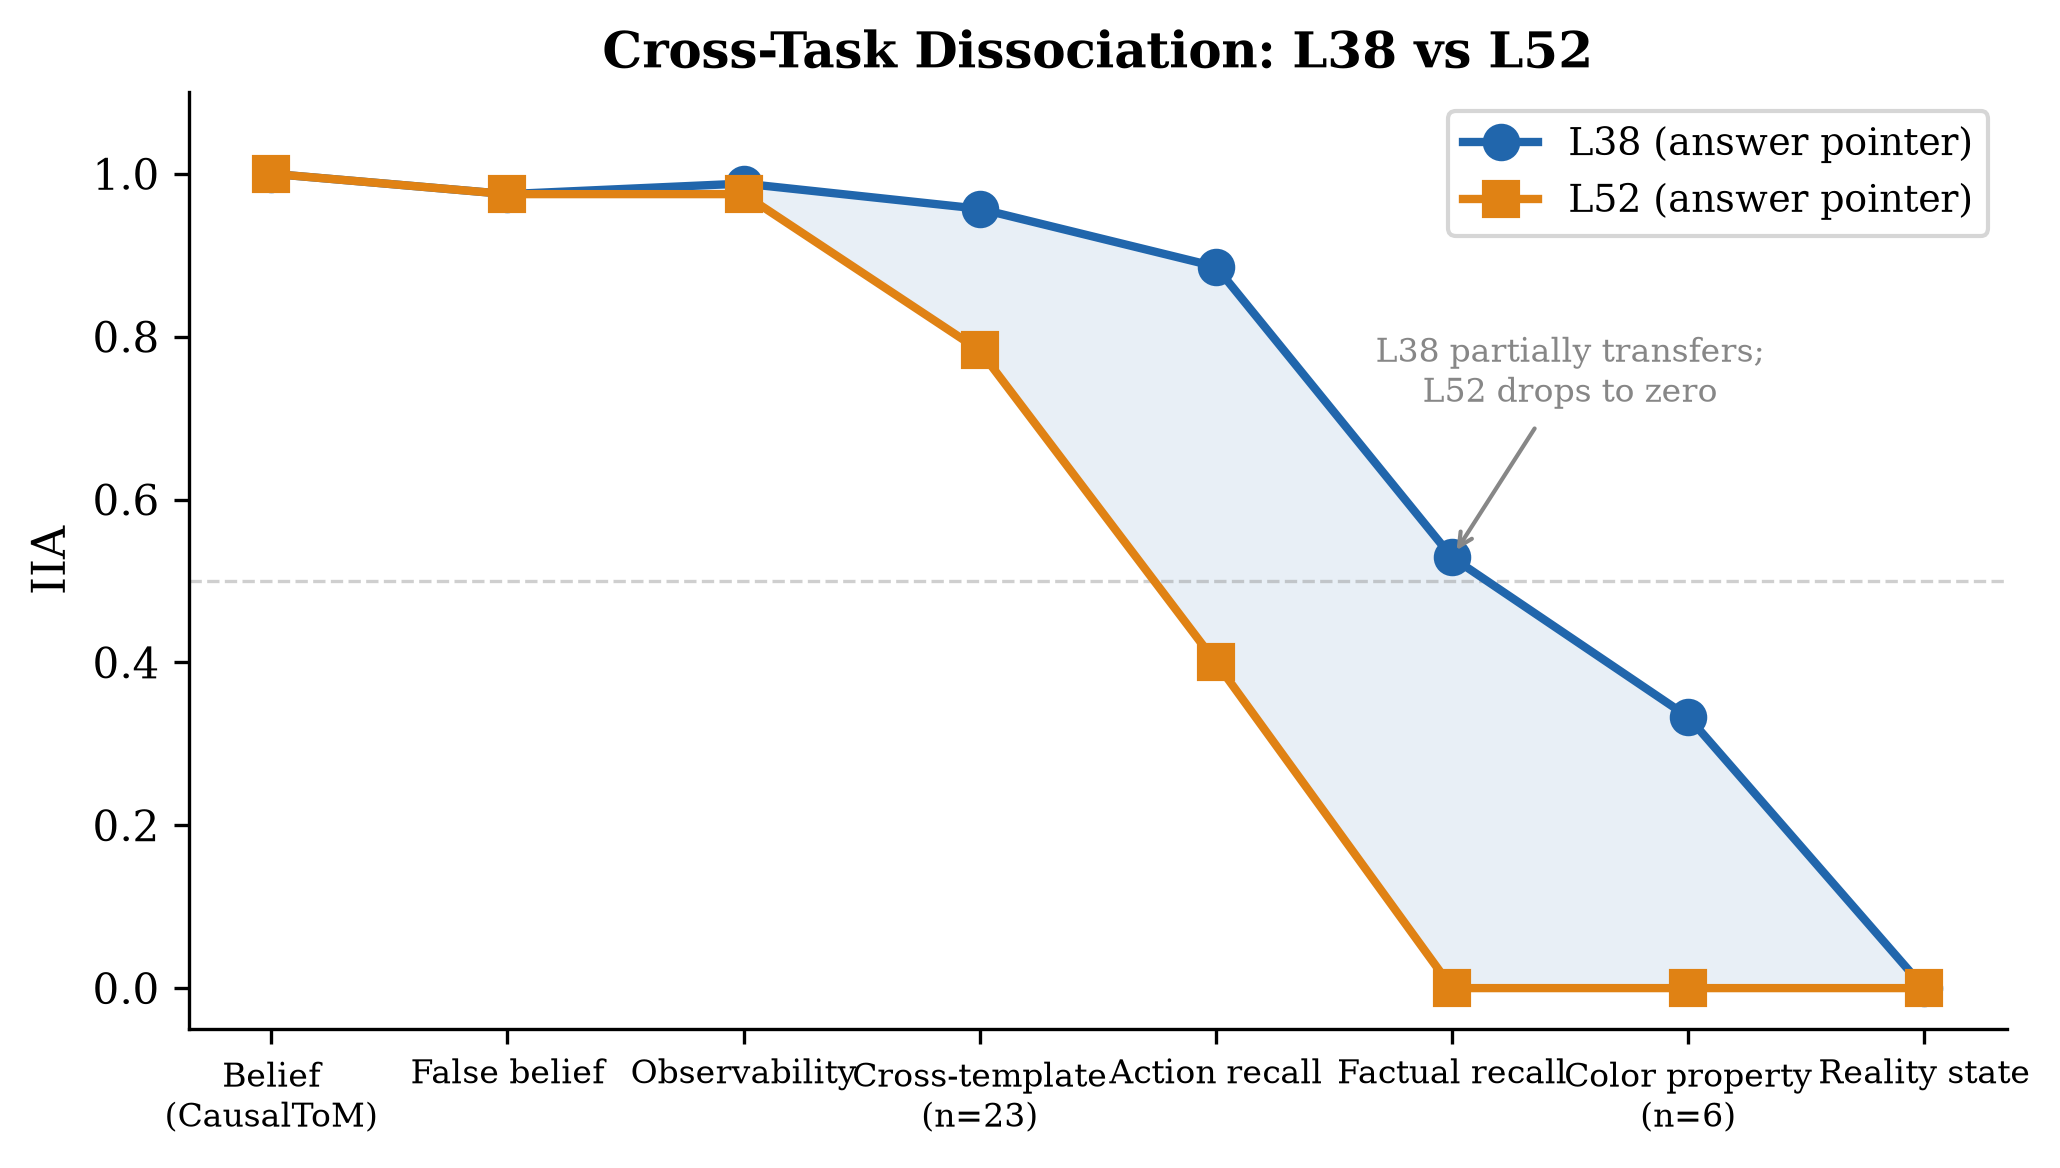
\includegraphics[width=\textwidth]{figures/fig5_crosstask.pdf}
\caption{Cross-task dissociation between L38 and L52. L38 partially transfers to factual recall (IIA $= 0.53$) and action recall (IIA $= 0.89$), while L52 drops to zero on non-belief tasks. Both subspaces achieve near-ceiling IIA on belief-relevant tasks (belief framing, false belief, observability). The gap between the two curves quantifies how much L38 acts as a generic retrieval mechanism compared to L52's task-specific function.}
\label{fig:crosstask}
\end{figure}

\subsection{Belief-vs-binding dissociation (EXP12--EXP15)}
\label{sec:dissociation_results}

Pre-registered in Amendment~9, these experiments test whether the subspaces encode generic entity-state bindings or character-perspective information.

\paragraph{EXP12: Question-framing control ($n = 35$ shared pairs).}
We generate clean/counterfactual pairs from the CausalToM template and reframe the question four ways, preserving the story and answer: \emph{belief} (``What does X believe the container contains?''), \emph{action recall} (``What did X put in the container?''), \emph{reality state} (``What is inside the container?''), \emph{fill completion} (``X filled the container with'').

Results in Table~\ref{tab:framing}. Under this selection rule the subspaces are framing-\emph{sensitive}: belief framing produces IIA $= 1.0$ across all subspaces, action recall yields partial transfer (L38 $= 0.886$, L52 $= 0.400$, L53 $= 0.057$), and reality-state and fill-completion framings produce IIA $= 0.0$. This \emph{overturns} our pre-registered prediction that all framings would be within $0.10$ of the belief baseline. Pre-committed interpretation: ``the subspace may be sensitive to epistemic question framing.'' The zeros do not survive per-framing filtering at $n = 250$ (Section~\ref{sec:partial}), so the effect this experiment supports is graded rather than categorical; both analyses are reported, with their selection rules, rather than one replacing the other.

If the subspaces encoded generic entity-state bindings (``what drink is in what container''), reality-state and fill-completion questions---which request the same underlying fact---should activate the same subspace. They do not. The subspaces encode information relevant specifically to character-perspective queries.

\begin{table}[t]
\centering
\caption{EXP12: IIA by question framing ($n = 35$ shared pairs) with 95\% Wilson confidence intervals, filtered on belief-question accuracy. Under that selection rule the subspaces respond to belief framing, partially to action recall, and not at all to reality or fill-completion queries. The $n = 250$ replication with per-framing filtering does not reproduce the zeros: reality-state reaches $0.82$--$0.916$ and action recall $0.98$--$1.0$ (Section~\ref{sec:partial}). Because the selection rule changed, these are different analyses rather than the same analysis at two sample sizes, and the categorical reading below belongs to this one. See Figure~\ref{fig:framing}.}
\label{tab:framing}
\begin{tabular}{lccc}
\toprule
\textbf{Framing} & \textbf{L38} & \textbf{L52} & \textbf{L53} \\
\midrule
Belief (``What does X believe\ldots'') & $1.00\ [.90, 1.0]$ & $1.00\ [.90, 1.0]$ & $1.00\ [.90, 1.0]$ \\
Action recall (``What did X put\ldots'') & $.89\ [.74, .96]$ & $.40\ [.25, .57]$ & $.06\ [.01, .19]$ \\
Reality state (``What is inside\ldots'') & $.00\ [.00, .10]$ & $.00\ [.00, .10]$ & $.00\ [.00, .10]$ \\
Fill completion (``X filled\ldots with'') & $.00\ [.00, .10]$ & $.00\ [.00, .10]$ & $.00\ [.00, .10]$ \\
\bottomrule
\end{tabular}
\end{table}

\begin{figure}[t]
\centering
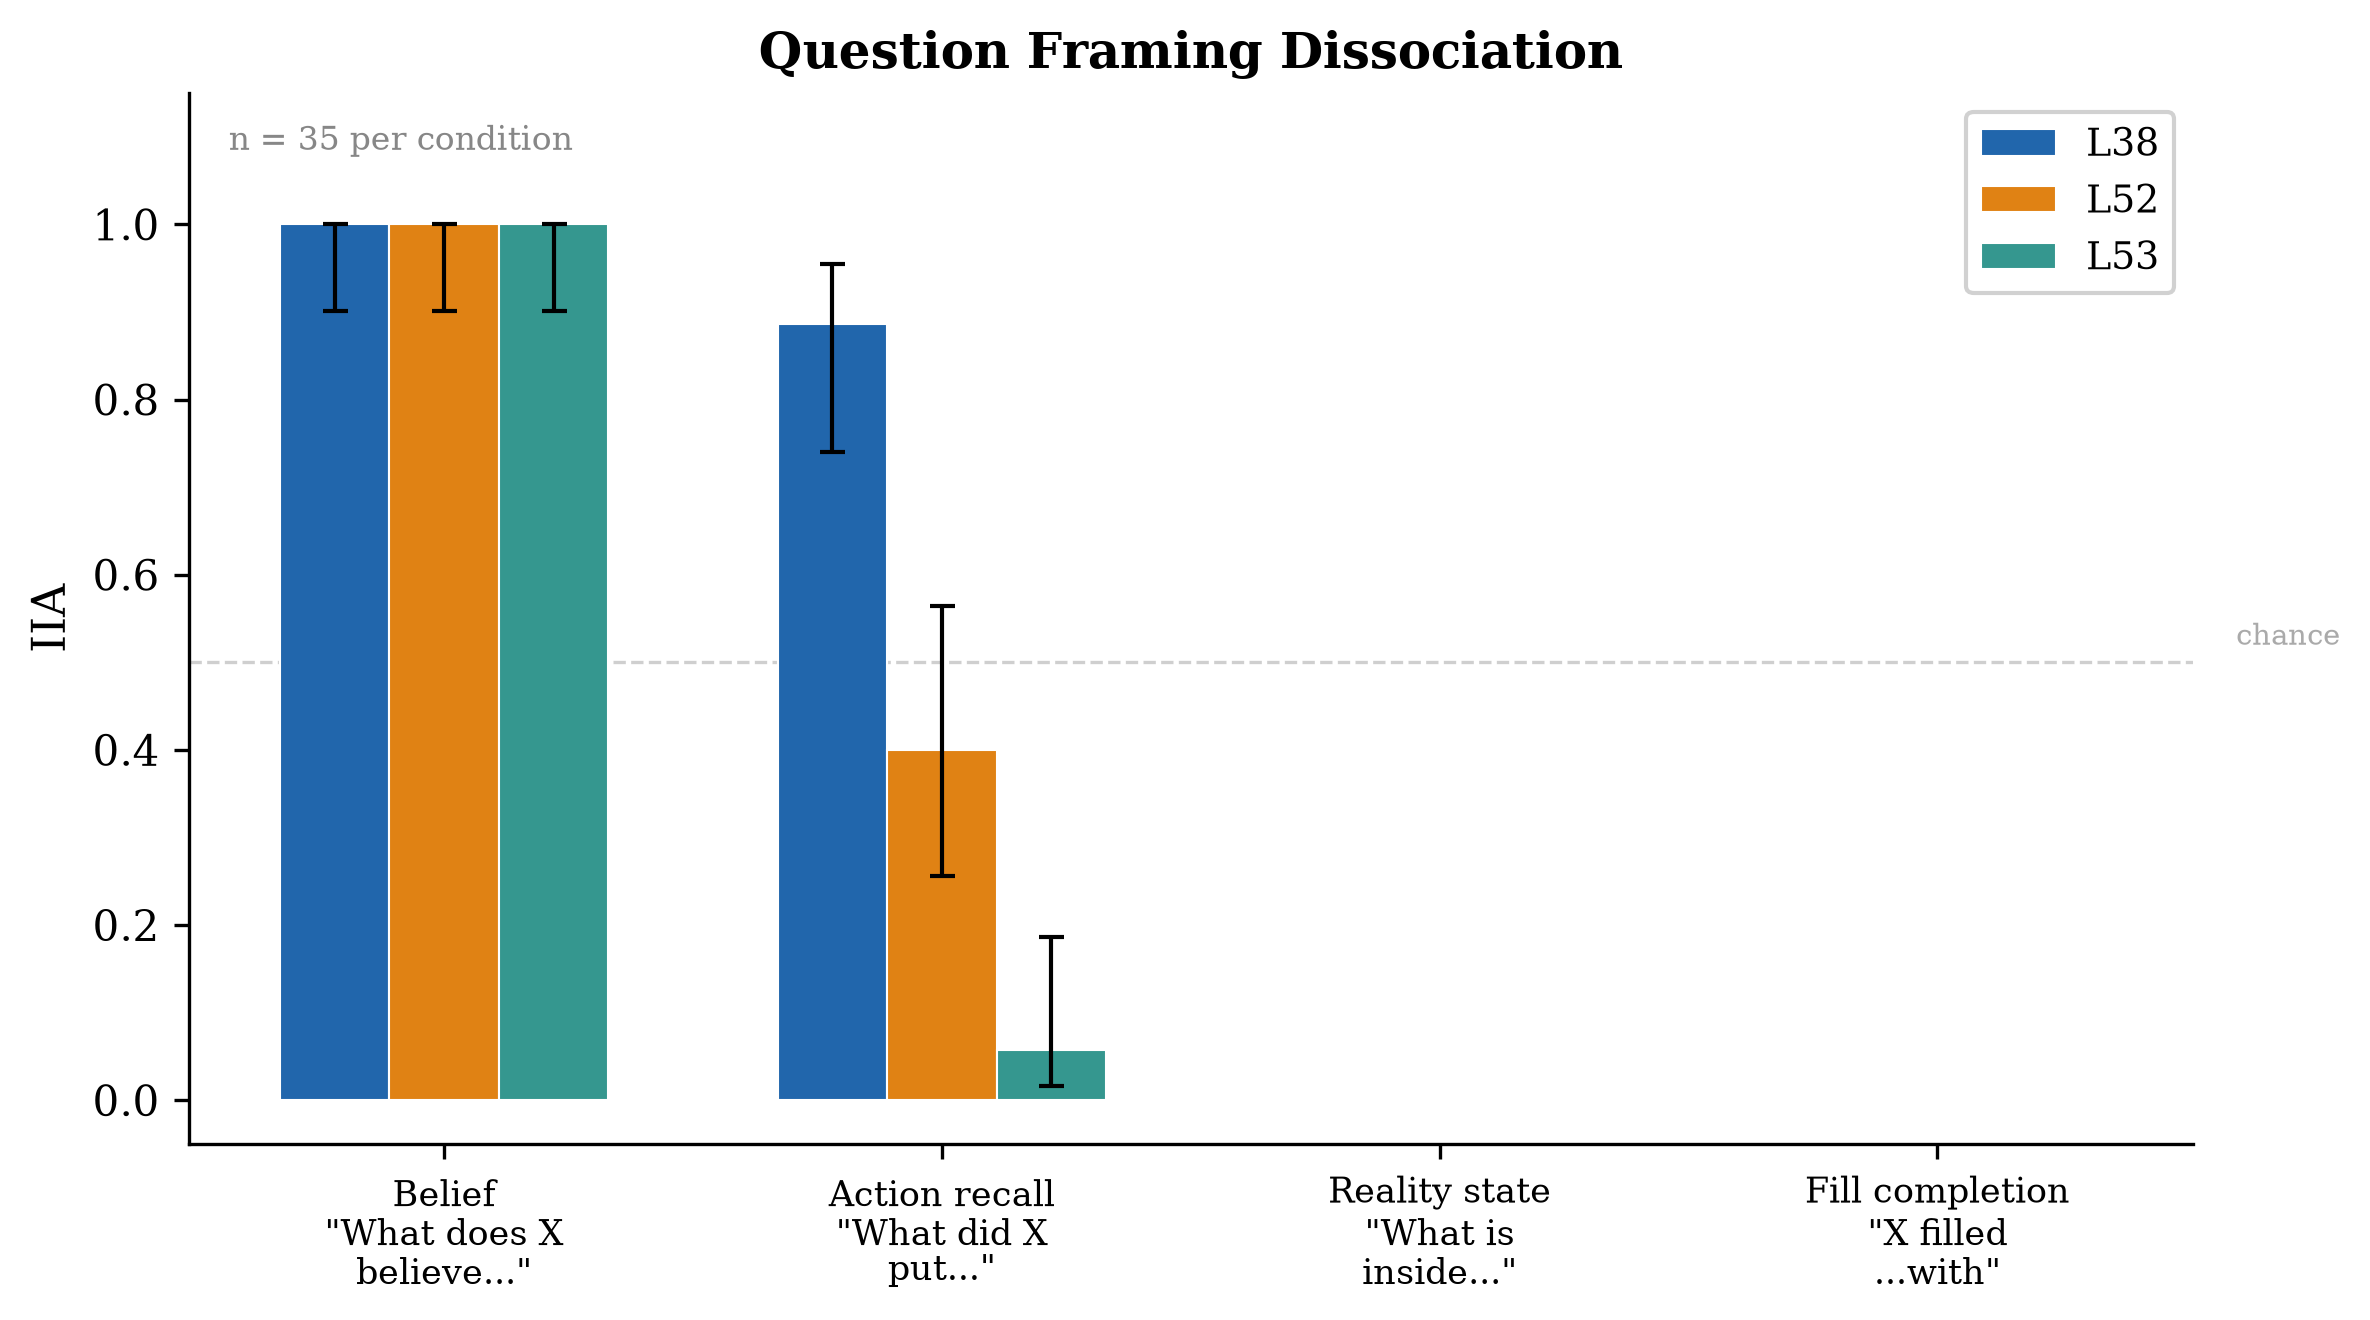
\includegraphics[width=\textwidth]{figures/fig2_framing_dissociation.pdf}
\caption{Question framing dissociation (EXP12, $n = 35$). The same clean/counterfactual story pairs produce IIA $= 1.0$ under belief framing, graded transfer under action recall (L38 $= 0.89$, L52 $= 0.40$), and IIA $= 0.0$ under reality-state or fill-completion framing. Error bars show 95\% Wilson confidence intervals. The underlying entity-state fact is identical across all four framings. At $n = 250$ with per-framing filtering the reality-state cell rises to $0.82$--$0.92$ (Section~\ref{sec:experiments}), so the effect the higher-powered design supports is graded rather than categorical.}
\label{fig:framing}
\end{figure}

\paragraph{EXP13: Distractor insertion ($n = 80$ baseline, $n = 21$ early, $n = 0$ mid/late).}
We insert irrelevant drink mentions at three positions: early (after scene-setting), mid (between fill actions), late (before the question). Baseline: L38/L52 IIA $= 1.0$, L53 $= 0.7$. Mid- and late-position distractors destroy behavioral accuracy entirely (zero surviving pairs). Early distractors retain 21 pairs, but IIA drops to $0.0$ across all subspaces. The subspace is positionally fragile: even minor template perturbations disrupt the mechanism. This limits the belief-tracking claim to the template structure used in training, though it does not bear on belief vs.\ generic retrieval.

\paragraph{EXP14: True false-belief test ($n = 80$, 100\% behavioral accuracy).}
A character places a drink, a second character swaps it unobserved, and the question asks what the first character \emph{believes} the container holds. The model answers all 80 correctly (reporting the original drink, not the swapped one).

The design leaves one alternative standing. In every pair the first character does not
observe the swap, so the belief-correct answer and the answer given by a surface rule
---\emph{a character who did not observe a change reports the state before it}---coincide on
all 80 items. Neither the behavioral filter nor IIA separates them, so the transfer reported
here is consistent with the subspaces carrying observation history rather than belief. The
condition that pulls them apart is one where the character is told about the swap:
belief then predicts the new state and the surface rule the old one. \citet{shapira2024clever}
construct the corresponding behavioral controls and find social-reasoning performance drops
sharply under them. We did not run it, and the false-belief result should be read under that
limit.

L38 and L52 both achieve IIA $= 0.975$ (95\% Wilson CI $[0.913, 0.993]$; L53 $= 0.388$). This \emph{overturns} our prediction of IIA $< 0.30$. Pre-committed interpretation: ``the subspace genuinely tracks the character's epistemic state even when it diverges from reality.'' Subspaces trained where belief equals reality generalize to stories where they diverge.

The reality-question control (asking what is \emph{actually} in the container) yielded zero viable pairs---the model could not reliably answer these. Uninformative.

\paragraph{EXP15: Observability dissociation ($n = 80$, 88\% behavioral accuracy).}
Template 1 creates an observability asymmetry: character 1 can observe character 2's actions, not vice versa. We ask character 1 about character 2's container (observed-other condition). The model answers 212 of 240 generated pairs correctly (88\%); we evaluate the first 80 passing pairs.

L38 IIA $= 0.988$ (95\% Wilson CI $[0.932, 0.998]$), L52 $= 0.975$ $[0.913, 0.993]$ (L53 $= 0.213$). Again overturns our prediction of IIA $< 0.30$. The subspaces generalize to knowledge acquired through observation, not just through the character's own actions.

The self-container control yielded zero viable pairs. Uninformative.

\subsection{Cross-model dependency structure}
\label{sec:crossmodel}

Prakash et al.'s cross-model appendix tests Qwen2.5-14B-Instruct and Llama-3.1-405B-Instruct with full-residual interchange interventions only, acknowledging that ``subspace interchange intervention experiments were not conducted'' yet concluding that these models ``employ the same underlying mechanism.'' Full-residual patching replaces all information at a position simultaneously and cannot distinguish address from payload.

We apply the paper's own three-condition mismatch test---their strongest causal design---to Qwen2.5-14B-Instruct ($n = 200$ pairs, 12 layers per lookback type). This test patches recalled tokens only (address updated, pointer stale), lookback tokens only (pointer updated, address stale), or both (coherent). The mismatch signature---singles fail, pair succeeds---demonstrates dependency structure without requiring subspace fitting.

\paragraph{Answer lookback: mismatch signature at layers 32--38.}
Recalled-only IIA $= 0.005$ $[0.001, 0.028]$, lookback-only IIA $= 0.000$ $[0.000, 0.019]$, both IIA $= 1.000$ $[0.981, 1.0]$ (95\% Wilson CIs, L32). The signature holds from L32 through L38 (67--79\% of Qwen's 48 layers). Layer 30 shows a transition (both $= 0.440$, singles near zero). The proportional depth is comparable to Llama-3-70B's answer range (layers 52--56, 65--70\% of 80 layers). Patching either component alone has no effect; patching both restores full counterfactual transfer.

\paragraph{Binding lookback: anti-mismatch.}
Recalled-only IIA $= 1.0$ across all layers (patching state tokens alone suffices). Lookback-only IIA rises from $0.0$ at L12 to $1.0$ by L24. From L24 onward, each component alone succeeds but the combined patch yields IIA $= 0.0$. The binding mechanism on Qwen does not require coordination between recalled and lookback positions---the combined patch creates an internally incoherent state. This is a genuine structural difference that full-residual patching cannot detect.

The answer lookback's dependency signature transfers to Qwen; the binding signature differs. That is a claim about the signature this test measures, not about whether the two models implement identical mechanisms, and the test fits no subspaces. What it shows is partial transport, which the paper's binary claim cannot express.

\subsection{Interaction structure of the mismatch test (reanalysis)}
\label{sec:interaction}

The mismatch test measures two token groups patched separately and together. With the
unpatched condition those are all four values of a two-player coalition function, so the
interaction between the groups is determined rather than estimated. Write
$x = (x_0, x_1) \in \{0,1\}^2$, where $x_0 = 1$ patches the recalled tokens and $x_1 = 1$
patches the lookback tokens, and let $v(x)$ be IIA against the counterfactual answer. Pairs
are filtered so the model returns the clean answer on the clean prompt, and the clean answer
differs from the counterfactual target by construction, so $v(0,0) = 0$ exactly. The
Walsh--Hadamard coefficients follow \citet{poelwijk2016context},
\begin{equation}
  w_S = \tfrac{1}{4} \sum_{x} v(x)\, (-1)^{\sum_{i \in S} x_i},
\end{equation}
with $w_2 \equiv w_{\{0,1\}}$ the deviation from additivity; positive is super-additive,
negative sub-additive. Because $v \in [0,1]$ with $v(0,0)$ pinned, $w_2$ reaches $-0.5$ when
both singles transfer perfectly and the pair transfers nothing, and $+0.25$ in the reverse
case, so a coefficient can be read as a fraction of the largest interaction the design admits.

\begin{table}[h]
\centering
\small
\caption{Order-2 Walsh coefficients for the two token groups, Qwen2.5-14B-Instruct,
$n = 200$ pairs per cell. Saturation is $w_2$ as a fraction of the bound it approaches.
Order-2 energy is the share of non-constant Walsh energy at order~2. Intervals resample cells
as independent binomials, which is not conservative: the dropped covariance terms have mixed
signs, so the reported width may be too narrow.}
\label{tab:interaction}
\vspace{0.5\baselineskip}
\begin{tabular}{llccccc}
\toprule
Mechanism & Layers & singles & pair & $w_2$ & saturation & order-2 energy \\
\midrule
Binding & 12--18 & $1.000$ / $0.010$ & $0.965$--$1.000$ & $-0.011$ & $0.02$ & $0.001$ \\
Binding & 20--22 & $1.000$ / $0.343$ & $0.425$--$0.445$ & $-0.227$ & $0.45$ & $0.399$ \\
Binding & 24--34 & $1.000$ / $0.999$ & $0.000$ & $-0.499$ & $1.00$ & $1.000$ \\
\midrule
Answer & 16--28 & $0.005$ / $0.000$ & $0.005$--$0.020$ & $+0.000$ & $0.01$ & $0.000$ \\
Answer & 30 & $0.010$ / $0.000$ & $0.440$ & $+0.108$ & $0.43$ & $0.323$ \\
Answer & 32--38 & $0.020$ / $0.010$ & $1.000$ & $+0.242$ & $0.97$ & $0.320$ \\
\bottomrule
\end{tabular}
\end{table}

\begin{figure}[h]
\centering
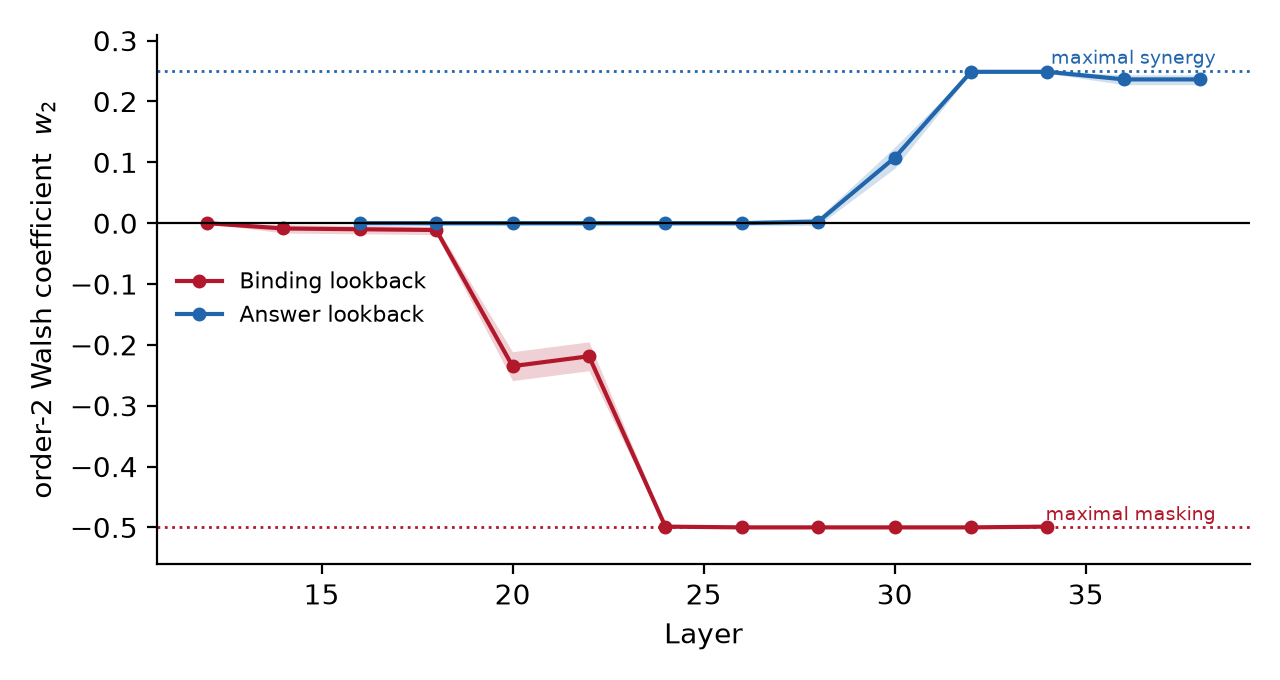
\includegraphics[width=0.68\textwidth]{figures/interaction_coefficient.pdf}
\caption{Order-2 Walsh coefficient by layer for the two lookback mechanisms in
Qwen2.5-14B-Instruct. Dotted lines mark the bounds the design admits. Binding reaches the
masking bound at layer 24 and holds it through layer 34; the answer lookback reaches $97\%$
of the synergy bound at layer 32 and holds it through layer 38. Shaded bands are 95\%
bootstrap intervals over $10{,}000$ draws.}
\label{fig:interaction}
\end{figure}

The two protocols return interactions of opposite sign, each saturated (Table~\ref{tab:interaction},
Figure~\ref{fig:interaction}). They are protocols rather than mechanisms because the two runs
differ in three respects at once, and the difference is not attributable among them. From layer 24 the binding coalition values are
$v = (0, 1, 1, 0)$ to within one pair in 200: either token group alone transfers the
counterfactual answer on every pair, both together transfer it on none. Both order-1
coefficients are exactly zero and $w_2 = -0.499$, so the function is parity over the two
groups and carries no additive component at all. From layer 32 the answer values are
$v = (0, 0.005, 0, 1)$: neither group transfers alone, together they transfer on every pair,
$w_2 = +0.249$ against a ceiling of $+0.25$, with the order-2 energy share of $0.331$ that a
conjunction takes. Sign stability across $10{,}000$ bootstrap draws is $1.000$ in every cell
above an additive tolerance of $0.01$. Neither pattern holds at the earliest layers tested:
binding is near-additive at layers 12--18 and passes through a mixed regime at 20--22, and the
answer lookback is flat until layer 30.

A summary reporting each token group's marginal contribution assigns the binding lookback two
zeros. The recalled tokens transfer the answer when the lookback tokens are untouched and
block it when they are patched, in compensating amounts, so the average over contexts is zero
and describes nothing that occurs at any layer. Read through marginals, binding at layer 26
and the answer lookback at layer 34 are both components of high causal relevance with clean
accuracy $1.0$; read through the interaction, one is parity and the other conjunction.
\citet{leemann2024slalom} prove attention cannot represent additive models over input tokens,
and \citet{tower2026epistatic} measures the component-level analogue for attention heads,
where functionally selected circuits carry $17$--$19\%$ of their coalition energy at order~2.

Three limits apply. The binding and answer runs are not a controlled comparison. They use
different counterfactual generators, are reported over different layer ranges, and---most
consequentially---patch lookback spans of different size: the binding protocol patches every
position from the question marker to the end of the prompt, while the answer protocol patches
the final position alone. Any of the three, span size included, could
account for the opposite signs; final-token-only patching has not been run on the binding pairs
at these layers, so none of them is established as the source. The results establish a
difference between the protocols as run. Separating its causes requires a crossed design at
shared layers with matched intervention size, which we have not run. Second, an order-2 share over two players is
not comparable to the same quantity over a fifteen-head circuit, so what carries weight in the
binding result is that the order-1 coefficients are exactly zero rather than that the share
reaches one. Third, \citet{benzer1955}
decides one unit or two from the sign of a double perturbation, sub-additivity reading as one
pathway; that convention was defined for loss-of-function perturbations, and interchange
interventions install a value rather than remove one, so we report the coefficients without
the same-unit verdict. The decomposition was derived from the cross-model results afterward and is a
follow-up rather than a registered prediction.

\subsection{Rescue reversibility (L38, $n = 200$)}

We zero-ablate the L38 answer subspace (rank 3) and measure five conditions: (A) clean baseline, (B) zero-ablated, (C) ablated then restored from original activation, (D) ablated then restored from a different sample, (E) ablated then restored with a random subspace of matched rank. Clean accuracy $= 1.0$; ablated $= 0.92$; rescued $= 1.0$; wrong-rescue $= 0.545$; random-rescue $= 0.93$. The ablation drop (8\%) is small---the model is robust to subspace removal, consistent with redundant pathways in the 8192-dimensional residual stream. The wrong-rescue drop to $0.545$ confirms the subspace carries sample-specific information: restoring the wrong sample's projection actively degrades performance below the ablated baseline. Random-subspace restoration ($0.93$) does not help, confirming directional specificity. The remaining answer subspaces (L52, L53) were not tested due to NDIF instability.

\subsection{Subspace ablation (I1, $n = 80$)}
\label{sec:ablation}

Zeroing each identified subspace ($x' = x - Px$) and rescoring accuracy separates carrying
information under interchange from being required for the behavior. Answer subspaces are
ablated at the final position, binding subspaces at all positions.

\begin{table}[h]
\centering
\small
\begin{tabular}{lrrrrc}
\toprule
subspace & rank & clean & ablated & drop & necessary \\
\midrule
binding L34 & 3 & 1.00 & 1.00 & 0.00 & no \\
binding L35 & 7 & 1.00 & 0.95 & 0.05 & no \\
binding L36 & 8 & 1.00 & 0.88 & 0.12 & yes \\
answer L38 & 3 & 1.00 & 0.93 & 0.07 & no \\
answer L52 & 18 & 0.96 & 0.86 & 0.10 & no \\
answer L53 & 19 & 1.00 & 0.89 & 0.11 & yes \\
\bottomrule
\end{tabular}
\caption{Accuracy under zero-ablation of each identified subspace, $n = 80$. A subspace is
recorded as necessary where removing it costs more than $0.10$ accuracy. Four of six fall
below that threshold, and removing L34 costs nothing measurable.}
\label{tab:ablation}
\end{table}

The same subspaces carry belief content under interchange at IIA near $1.0$. Sufficiency to
drive the behavior and necessity for it come apart here: a subspace whose replacement changes
the answer, and whose removal does not, is engaged by the intervention without being required
by the model's own forward pass. \citet{makelov2024illusion} describe a mechanism by which
this arises, where a subspace intervention recruits a pathway that is dormant in normal
operation; \citet{wu2024replyillusion} argue that the condition they use to detect it holds
too widely to be diagnostic. We report the dissociation rather than adjudicating that
dispute. The measurement that would separate the readings is whether these directions vary
with belief state and predict behavior with no intervention at all, which this design does
not test.

\subsection{Experiments with partial or incomplete results}
\label{sec:partial}

\paragraph{EXP12v2: Question-framing replication ($n = 250$ shared pairs, partial).}
We rerun the question-framing control at $n = 250$ with per-framing accuracy filtering. Belief framing confirms the $n = 35$ result: IIA $= 1.0$ for all three subspaces (L38 $[0.985, 1.0]$, L52 $[0.985, 1.0]$, L53 $[0.985, 1.0]$). Action recall shows IIA near ceiling (L38 $= 0.98$, L52 $= 1.0$, L53 $= 1.0$), higher than the $n = 35$ result (L38 $= 0.886$, L52 $= 0.400$, L53 $= 0.057$). This shift is attributable to a methodological difference: the $n = 250$ design filters pairs per-framing (requiring model accuracy under each framing before computing IIA), then intersects, whereas the $n = 35$ design filtered on belief framing only. Per-framing filtering selects stories where the model handles action recall well, biasing the action-recall IIA upward. The choice to filter per framing was made after the $n = 35$ result was seen, so it is a post-hoc analysis decision on the experiment that carries the framing claim, and both analyses are reported here for that reason.

Reality-state completed at $n = 250$ and gives IIA $= 0.916$ (L38, $k = 229/250$, $[0.875, 0.944]$), $0.82$ (L52, $k = 205/250$) and $0.82$ (L53). This is a reliable reduction from the belief condition on non-overlapping intervals, and it is not the absence of transfer the $n = 35$ analysis reported. The same per-framing filtering that raised action recall to ceiling raises reality-state from near zero to $0.82$--$0.92$, so the four-way dissociation as originally described does not survive the higher-powered design. What survives is a graded framing effect. Fill-completion has not been computed at $n = 250$ and is the remaining cell.

\paragraph{Remaining incomplete experiments.}
EXP8 (layer spread): filtered pairs cached but no IIA computed. EXP6 (cross-stage mediation): every condition returned \texttt{nan}, so neither the forward nor the backward effect is estimated and the unity of the three sub-mechanisms is untested. The analysis script reported ``independent processes'' from that run, a verdict produced by comparisons against \texttt{nan} rather than by data; it carries no weight here. M1 (dose-response graded ablation): filtered pairs cached, no graded results. EXP9 (rank decomposition): the per-direction intervention produced zero IIA at all ranks including full-rank reconstruction, despite the original subspace achieving IIA $> 0.9$---a methodology failure in the per-direction intervention, not a scientific finding. EXP4 (surface heuristic) and EXP5 (compositional generalization): only dry-run or zero-pair results. These experiments do not affect the central conclusions, which rest on EXP1 (replication), EXP10--EXP11 (specificity), EXP12--EXP15 (the belief-vs-binding dissociation), and the cross-model dependency structure.

\subsection{Confounding sensitivity (I8, exploratory)}

We compute E-values \citep{vanderweele2017sensitivity} for all 20 positive effects (IIA $>$ baseline) to assess robustness to unmeasured confounders. $E = \text{RR} + \sqrt{\text{RR} \cdot (\text{RR} - 1)}$, where $\text{RR} = \text{IIA} / \text{baseline}$ and baseline $= 0.5$ (chance under random subspace swap).

19 of 20 achieve $E \geq 2.0$ (Figure~\ref{fig:evalues}). The single fragile effect is L38 on factual recall ($E = 1.31$, IIA $= 0.529$), consistent with L38's partial cross-task transfer (EXP11). Replication, false belief, observability, and belief framing achieve $E = 3.31$--$3.41$. This analysis was added after initial pre-registration (Amendment~10c) and is exploratory.

\begin{figure}[t]
\centering
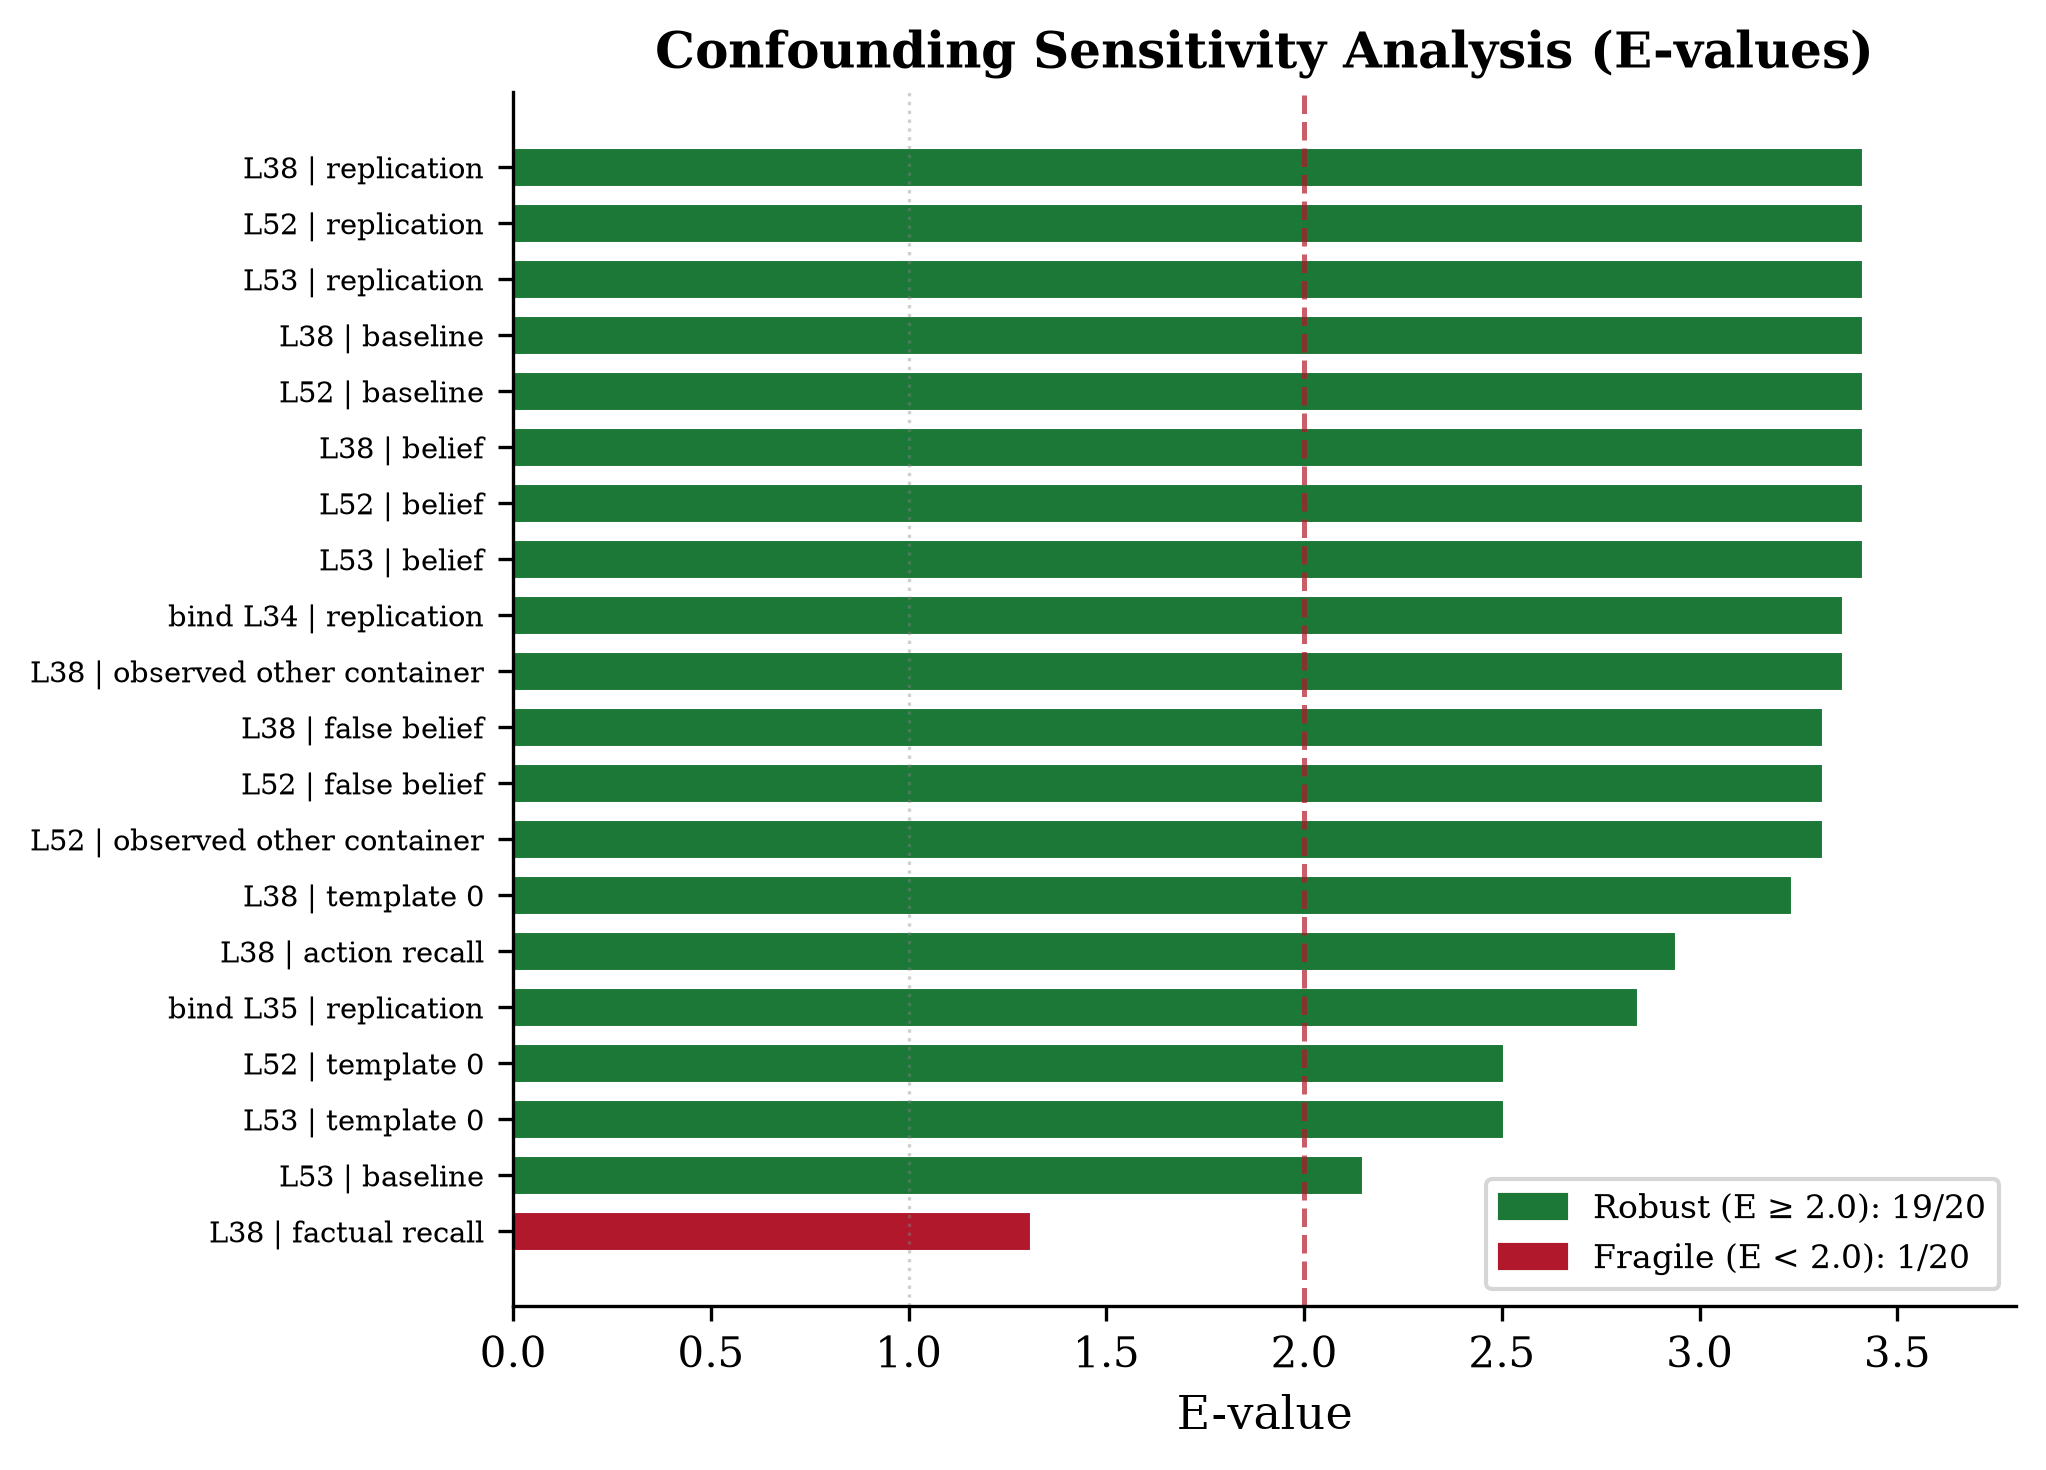
\includegraphics[width=\textwidth]{figures/fig3_evalues.pdf}
\caption{Confounding sensitivity analysis (I8, exploratory). E-values for all 20 positive effects (IIA $>$ chance), sorted by magnitude. An E-value quantifies how strong an unmeasured confounder would need to be to explain away the observed effect. The dashed line marks $E = 2.0$; effects above this threshold are considered robust. Only one effect falls below: L38 on factual recall ($E = 1.31$), consistent with L38's partial cross-task transfer.}
\label{fig:evalues}
\end{figure}

\subsection{Summary}

Figure~\ref{fig:heatmap} summarizes IIA across all completed experiments.

\begin{figure}[t]
\centering
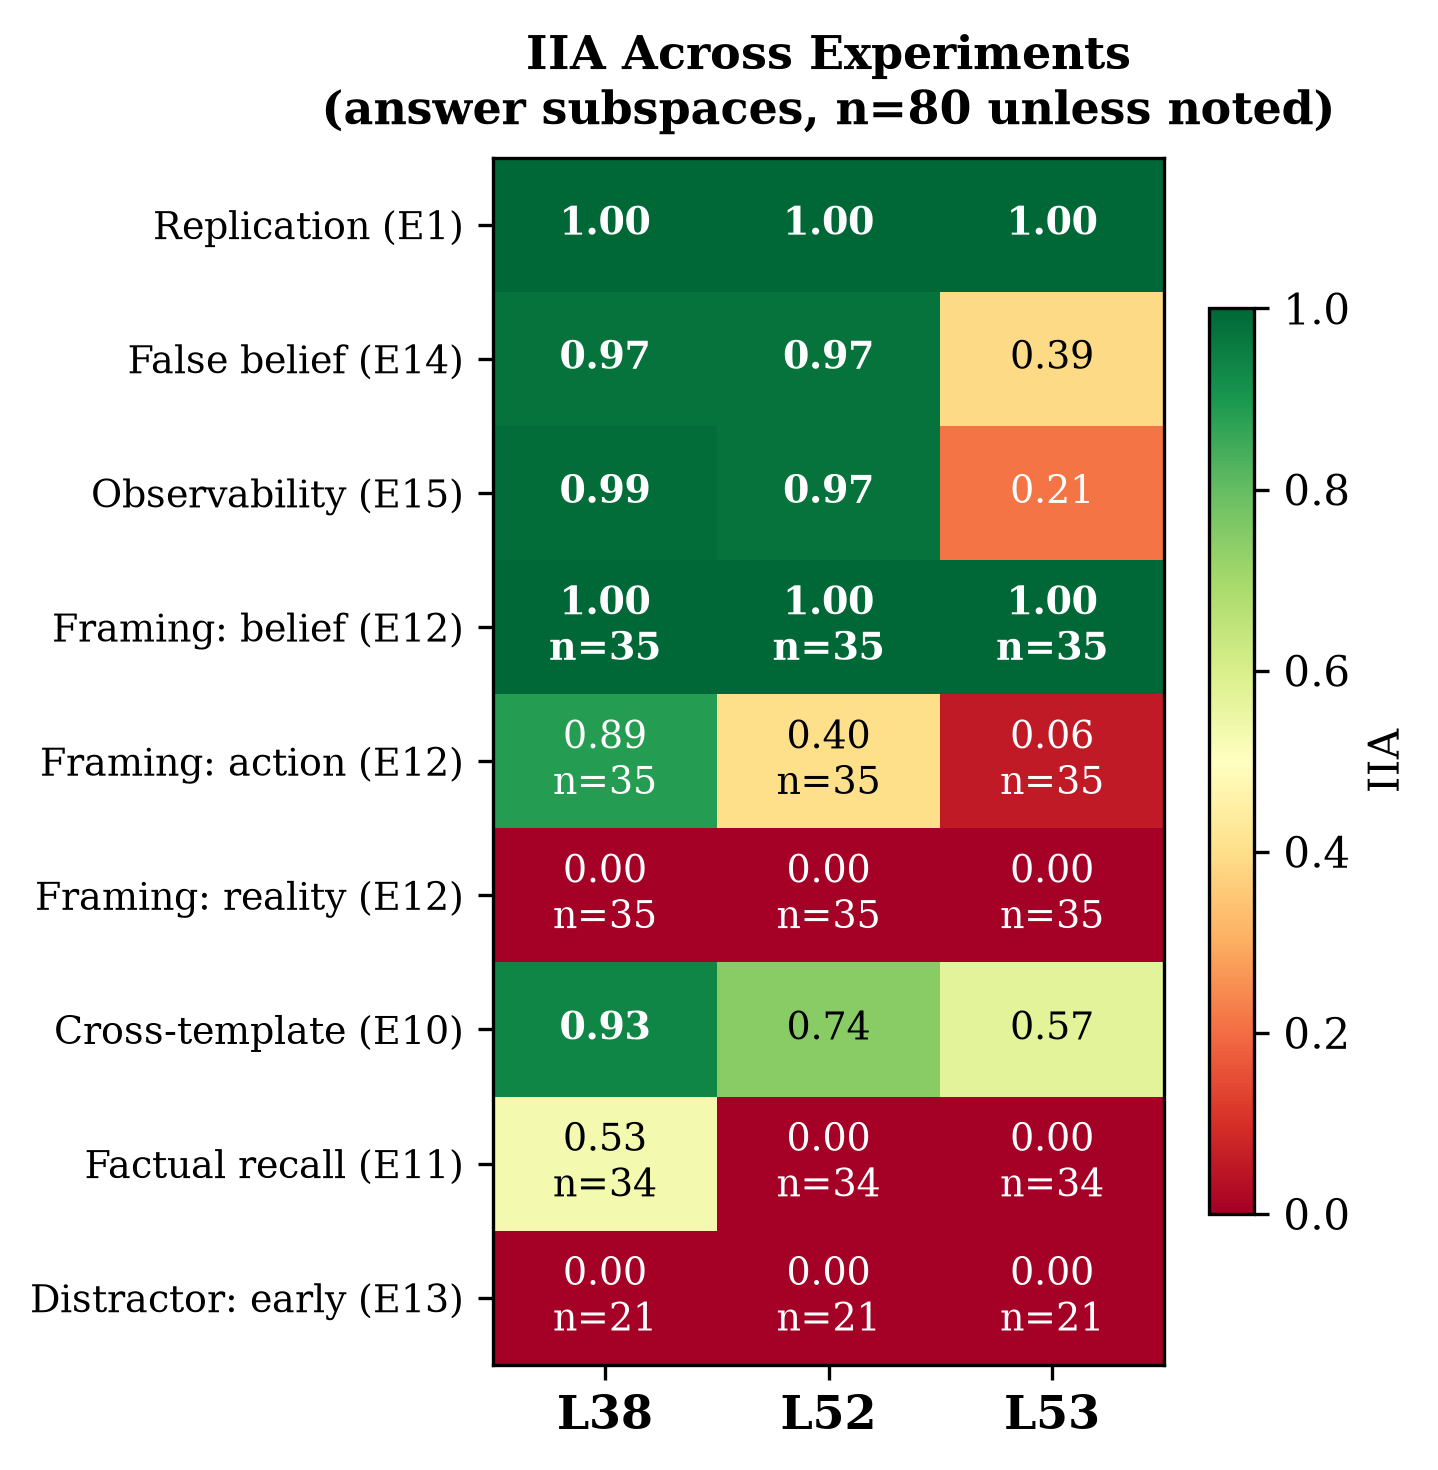
\includegraphics[width=0.75\textwidth]{figures/fig1_iia_heatmap.pdf}
\caption{IIA across all completed experiments for the three answer-pointer subspaces. L38 and L52 achieve near-ceiling IIA on belief-relevant tasks (replication, false belief, observability, belief framing). The reality-state and fill-completion cells shown here are the $n = 35$ values; the $n = 250$ replication with per-framing filtering gives reality-state $0.82$--$0.92$ and is reported in Section~\ref{sec:experiments}. L53 is unreliable across conditions, consistent with its high seed-to-seed variance (EXP1). Factual recall transfers partially to L38 (0.53) but not L52/L53, supporting the L38-as-generic-retrieval interpretation. All sample sizes are $n = 80$ unless noted.}
\label{fig:heatmap}
\end{figure}

\begin{table}[t]
\centering
\caption{Summary of pre-registered experiments with completed results. Predictions marked with $\dagger$ were overturned by the data in the audited claim's favor. EXP13's prediction was also overturned, in the other direction: we predicted robustness to distractors and found fragility. The dagger marks direction, not merely surprise. L53 is excluded from the verdict column due to high seed-to-seed variance (EXP1).}
\label{tab:summary}
\begin{tabular}{lp{3.2cm}p{3.2cm}l}
\toprule
\textbf{Exp.} & \textbf{Prediction} & \textbf{Result (L38/L52)} & \textbf{Verdict} \\
\midrule
EXP1 & Replicates within $\pm 0.05$ & L34: $+0.025$; L38/L52: higher & Passes \\
EXP10 & Cross-template transfer & L38: $0.957$ & Passes \\
EXP11 & No cross-task transfer & L38: $0.529$; L52: $0.0$ & Mixed \\
EXP12$^\dagger$ & Framing-invariant & Graded framing effect & Partial \\
Cross-model & Same mechanism cross-model & Answer transfers, binding differs & Partial \\
Rescue & Rescue recovers accuracy & 8\% drop, rescue to 1.0 & Partial \\
EXP13 & Robust to distractors & Fragile ($n=0$ mid/late) & Fails \\
EXP14$^\dagger$ & False-belief IIA $< 0.30$ & IIA $= 0.975$ & Overturned \\
EXP15$^\dagger$ & Observed-other IIA $< 0.30$ & IIA $= 0.988$ & Overturned \\
\bottomrule
\end{tabular}
\end{table}


\section{Discussion}
\label{sec:discussion}

We did not predict this verdict. We expected the subspaces to encode generic entity-state bindings that happen to align with beliefs on the paper's task. Three of four dissociation experiments overturned their pre-registered predictions, each time \emph{strengthening} the paper's claim.

EXP14 is the strongest result. CausalToM instantiates no false belief, and its own templates show the omission: \texttt{story\_templates.json} defines a \texttt{causal\_event} field carrying the unobserved swap, and \texttt{Dataset.set\_story()} (\texttt{src/dataset.py:73}) assigns \texttt{self.story = self.template["context"]} without ever reading it. Queries also always concern a character's own container (\texttt{set\_character=rc, set\_container=rc}), so belief equals reality for every pair. Appendix~M of the paper does report false-belief experiments, on BigToM, and also reports that its subspaces are not shared with CausalToM's---so the subspaces audited here were identified where no false belief occurs. We constructed 80 stories with genuine drink swaps that the queried character does not observe. The model answers all 80 correctly (reporting the believed drink, not the swapped one), and the subspaces achieve IIA $= 0.975$ at L38 and L52. The directions learned entirely from true-belief stories carry false-belief content---evidence the paper never collected.

EXP15 extends this. We ask a character about a container filled by someone else, where the queried character observed the filling. L38 IIA $= 0.988$, L52 $= 0.975$. The mechanism generalizes to knowledge acquired through observation, not just through the character's own actions.

EXP12 is most informative. We predicted framing-invariance: belief, action-recall, reality-state, and fill-completion questions would produce matched IIA, indicating generic entity-state lookup. The opposite occurred. At $n = 35$ the subspaces looked silent under perspective-free framing, and at $n = 250$ with
per-framing filtering they are not: belief gives IIA $= 1.0$, action recall $0.98$--$1.0$, and
reality-state $0.82$--$0.92$ over the same story pairs. The underlying entity-state
fact---which drink is in which container---is identical across all four framings, so the
effect the higher-powered design supports is graded rather than categorical. Framing costs
transfer; it does not abolish it.

That weakens the reading the $n = 35$ result invited. The subspaces are not silent on
``what entity is associated with what state,'' so framing-sensitivity alone does not
establish that they encode something perspective-specific. What the evidence supports is
that they are read out more effectively under character-perspective queries, and that they
update when characters observe events (EXP15) and transfer to stories where belief diverges
from reality (EXP14), subject to the confound noted there. Referential inflation (Section~\ref{sec:validity}) was warranted as an a priori worry, but the mechanism is more specific than generic retrieval.

\paragraph{The L38 vs.\ L52/L53 dissociation.}
L38 partially transfers to factual recall (EXP11: IIA $= 0.529$) and generalizes across templates (EXP10: IIA $= 0.957$; Figure~\ref{fig:crosstask}). L52 and L53 show zero transfer to non-belief tasks. L38 also shows the strongest transfer to action-recall framing (EXP12: $0.886$ vs.\ L52's $0.400$). This suggests L38 encodes a more generic entity-retrieval mechanism that the belief circuit routes through, while L52 is task-specific. The paper's three-stage architecture (binding $\to$ answer $\to$ visibility) may be better characterized as: generic retrieval (L38) feeding into task-specific formatting (L52/L53) feeding into input gating (visibility layers). L53 is unreliable: seed-to-seed variance is high (EXP1: the paper reports $0.55$ at seed 10; we observe $1.0$ at seed 42).

\paragraph{Positional fragility.}
EXP13 reveals positional fragility: minor template perturbations destroy behavioral accuracy (mid/late: zero surviving pairs) or subspace function (early: IIA $= 0.0$). The belief-tracking claim holds within the training template structure; the mechanism may not survive naturalistic text.

\paragraph{Incomplete experiments.}
EXP4--EXP9 could not be completed due to NDIF server instability and model-accuracy filtering; compositional generalization (EXP5) is withdrawn rather than deferred. Its stimuli yielded no viable pairs, and the question was answered at larger scale before we re-ran it: \citet{gurarieh2025mixing} evaluate the positional mechanism across nine models and ten tasks and report that it does not generalize beyond settings with two or three entity groups, offering lexical and reflexive retrieval as alternative mechanisms. Those are rival explanations this audit did not consider under I5.

\paragraph{Scope.}
All Llama experiments use one model (Llama-3.1-70B-Instruct, a minor version update from the paper's Llama-3-70B-Instruct). The cross-model test extends to Qwen2.5-14B-Instruct, where the answer lookback dependency structure transfers but the binding mechanism operates differently. We use the paper's released SVD bases and masks rather than recomputing them, so our results test \emph{generalization} to novel stimuli rather than \emph{replicability} from scratch. Two controls returned nothing and are reported as uninformative: the self-container control and EXP14's reality-question control both yielded zero viable pairs. Separately, EXP12v2's reality-state \emph{framing} condition yielded 250 shared pairs under per-framing filtering (Section~\ref{sec:experiments}); it is a different comparison and does not resolve the reality-question control.

\paragraph{Verdict.}
We issue a verdict per reading rather than one for the claim. Table~\ref{tab:readings}
records five readings the audited paper's evidence and ours bear on differently.

\begin{table}[h]
\centering
\small
\begin{tabular}{p{7.4cm}l}
\toprule
reading & verdict \\
\midrule
The answer lookback at L38 and L52 retrieves belief-conditioned content in
Llama-3.1-70B-Instruct & Causally Suggestive \\
The subspaces encode belief rather than observation history & Underdetermined \\
The three sub-mechanisms constitute one lookback mechanism & Underdetermined \\
The same mechanism operates across models & Disconfirmed \\
The identified subspaces are required for the behavior & Disconfirmed \\
\bottomrule
\end{tabular}
\caption{Verdicts by reading. The first is primary. Two readings are underdetermined
because the evidence that would settle them was not collected: in every false-belief story
the character fails to observe the swap, so belief and observation history name the same
answer, and the cross-stage test that would establish the three-way carving returned no
usable estimates. Two are disconfirmed on evidence reported here rather than absent from
the record.}
\label{tab:readings}
\end{table}

The two disconfirmed readings are not gaps. A single grade over ``the lookback mechanism''
would assert that its three sub-mechanisms are one thing, which is what C6 records as
unestablished: they are ablated singly, the cross-stage experiment that would test the
carving returned no usable estimates, and the cross-model test finds the answer dependency structure
transporting to Qwen2.5-14B-Instruct while binding does not. Grading the whole would
therefore claim in the verdict what the audit declines to claim in the criteria.

The evidence assembled here is substantial and it does not move the tier. The subspaces
replicate on a minor model version update (Figure~\ref{fig:replication}), are absent on
non-belief tasks at L52 and L53 (construct validity), generalize to false beliefs and to
observability-mediated knowledge (external validity), and are framing-sensitive rather than
framing-invariant, with reality framing costing transfer without abolishing it (interpretive
validity, Figure~\ref{fig:framing}). Baseline separation is now among them. M2 asks whether a
matched-rank random subspace achieves comparable interchange accuracy, and EXP2 answers it
directly: none of 350 random draws reaches the identified value at any of the six subspaces.
The rescue control agrees from the other direction, since restoring an ablated L38 from a
random subspace of matched rank recovers $0.93$ against an ablated floor of $0.92$ and a
true-subspace rescue of $1.0$. We record M2 as established, which opens the causal rungs
rather than closing the question: the gates that then bind are E1, since every story follows
one template, and I4, where cross-task transfer at L38 and fragility under distractor
insertion point in opposite directions.

All three answer subspaces therefore stay at \textbf{Causally Suggestive}, as does binding.
Under zero-ablation the same subspaces are largely dispensable (Table~\ref{tab:ablation}),
so what the interchange evidence supports is that these directions are sufficient to redirect
the answer, not that the model requires them. What now holds them there is not one
experiment but two gaps: a prompt distribution beyond the single template (E1), and a rival
account of the same transfer excluded rather than left standing (I4). Reaching ``Triangulated''
beyond that would require convergent evidence from an independent method (weight analysis,
probing), a measurement of these directions without intervention, and cross-model replication
with multi-seed statistics.

\paragraph{Convergent evidence from the authors' own later work.}
\citet{cui2026dual}, four of whose authors are authors of the audited paper, extend the
binding account to vision-language models and report two concurrent mechanisms for spatial
variable binding. The one carried by the language-model backbone, the analogue of the
mechanism audited here, ``plays only a secondary role in shaping model predictions,'' while
the dominant spatial signal originates in the vision encoder. That is the same shape as the
cross-model result reported in Section~\ref{sec:crossmodel}: a binding mechanism identified
by intervention, which turns out to carry less of the computation than its name implies once
a second setting is examined.

\paragraph{Future work.}
Three extensions follow from the design rather than from its results. The first is a full
36-criterion scorecard in the framework's own schema, where each status is derivable from a
verbatim quotation with a locator in the audited source, and a criterion with no quotation is
recorded as an assertion rather than a result. The second is binding every reported figure to
the run that produced it, so a number in this manuscript and a number in a results file
cannot disagree; three completed experiments in this audit were absent from an earlier draft
because no such binding existed. The third is a second case: \citet{cui2026dual} apply the
binding account in another modality, and auditing it against the same criteria would test
whether the verdicts here are a property of the claim or of the auditor.

\paragraph{Revised claim.}
We originally proposed contracting ``belief tracking via pointer dereference'' to ``attention-mediated retrieval.'' EXP12--EXP15 warrant a more specific characterization. The subspaces encode character-state associations that update with observability and state changes, accessible specifically through character-perspective queries. This is richer than ``retrieval'' but more precise than ``belief tracking''---belief tracking implemented as entity-state binding, not as a separate cognitive primitive. We propose the term \emph{perspective-indexed entity binding}: the bindings are indexed to
whose perspective a question asks about, and are read out differently under belief framing
than under reality framing. We do not call them belief-constitutive. Constitution is a
non-causal relation, and the standard test for constitutive relevance in the mechanism
literature is mutual manipulability, which requires intervening on the mechanism and on the
phenomenon in both directions; the cross-stage experiment that would supply the second
direction returned no usable estimates. The ablation result runs the other way, since a
subspace whose removal costs at most $0.12$ accuracy is a poor candidate for what the answer
consists in. V1 and V4 are the two criteria this audit records as outright failures against
its target, and a term asserting a relation the evidence does not reach would repeat them.

\paragraph{Implications for mechanistic interpretability.}
Because these predictions were pre-registered, the pattern of overturned predictions is itself evidence: we designed experiments to find entity binding and found belief tracking instead. EXP12, which we expected to undermine the paper's interpretation, returned a graded effect in its favor instead.


\section*{Data and Code Availability}

All audit materials, pre-registration documents, and experiment code are available at \url{https://github.com/elliottower/lookback-validity-audit}.

\bibliographystyle{tmlr}
\bibliography{references}

\end{document}
